% Options for packages loaded elsewhere
\PassOptionsToPackage{unicode}{hyperref}
\PassOptionsToPackage{hyphens}{url}
%
\documentclass[
  12pt,
  a4paper]{article}
\usepackage{lmodern}
\usepackage{amsmath}
\usepackage{ifxetex,ifluatex}
\ifnum 0\ifxetex 1\fi\ifluatex 1\fi=0 % if pdftex
  \usepackage[T1]{fontenc}
  \usepackage[utf8]{inputenc}
  \usepackage{textcomp} % provide euro and other symbols
  \usepackage{amssymb}
\else % if luatex or xetex
  \usepackage{unicode-math}
  \defaultfontfeatures{Scale=MatchLowercase}
  \defaultfontfeatures[\rmfamily]{Ligatures=TeX,Scale=1}
\fi
% Use upquote if available, for straight quotes in verbatim environments
\IfFileExists{upquote.sty}{\usepackage{upquote}}{}
\IfFileExists{microtype.sty}{% use microtype if available
  \usepackage[]{microtype}
  \UseMicrotypeSet[protrusion]{basicmath} % disable protrusion for tt fonts
}{}
\makeatletter
\@ifundefined{KOMAClassName}{% if non-KOMA class
  \IfFileExists{parskip.sty}{%
    \usepackage{parskip}
  }{% else
    \setlength{\parindent}{0pt}
    \setlength{\parskip}{6pt plus 2pt minus 1pt}}
}{% if KOMA class
  \KOMAoptions{parskip=half}}
\makeatother
\usepackage{xcolor}
\IfFileExists{xurl.sty}{\usepackage{xurl}}{} % add URL line breaks if available
\IfFileExists{bookmark.sty}{\usepackage{bookmark}}{\usepackage{hyperref}}
\hypersetup{
  pdftitle={Spatial Data Visualization and Analytics (Full Course Material)},
  pdfauthor={Ujaval Gandhi},
  hidelinks,
  pdfcreator={LaTeX via pandoc}}
\urlstyle{same} % disable monospaced font for URLs
\usepackage[margin=1in]{geometry}
\usepackage{longtable,booktabs}
\usepackage{calc} % for calculating minipage widths
% Correct order of tables after \paragraph or \subparagraph
\usepackage{etoolbox}
\makeatletter
\patchcmd\longtable{\par}{\if@noskipsec\mbox{}\fi\par}{}{}
\makeatother
% Allow footnotes in longtable head/foot
\IfFileExists{footnotehyper.sty}{\usepackage{footnotehyper}}{\usepackage{footnote}}
\makesavenoteenv{longtable}
\usepackage{graphicx}
\makeatletter
\def\maxwidth{\ifdim\Gin@nat@width>\linewidth\linewidth\else\Gin@nat@width\fi}
\def\maxheight{\ifdim\Gin@nat@height>\textheight\textheight\else\Gin@nat@height\fi}
\makeatother
% Scale images if necessary, so that they will not overflow the page
% margins by default, and it is still possible to overwrite the defaults
% using explicit options in \includegraphics[width, height, ...]{}
\setkeys{Gin}{width=\maxwidth,height=\maxheight,keepaspectratio}
% Set default figure placement to htbp
\makeatletter
\def\fps@figure{htbp}
\makeatother
\setlength{\emergencystretch}{3em} % prevent overfull lines
\providecommand{\tightlist}{%
  \setlength{\itemsep}{0pt}\setlength{\parskip}{0pt}}
\setcounter{secnumdepth}{-\maxdimen} % remove section numbering
\usepackage{fontspec}
\setmainfont[Ligatures=TeX]{lmodern}
\usepackage{fancyhdr}
\pagestyle{fancy}
\renewcommand{\footrulewidth}{0.4pt}
\fancyhead[LE,RO]{\thepage}
\geometry{left=1in,top=0.75in,bottom=0.75in}
\fancyfoot[CE,CO]{{
\includegraphics[height=0.5cm]{images/cc-by-nc.png}} Ujaval Gandhi http://www.spatialthoughts.com}
\ifluatex
  \usepackage{selnolig}  % disable illegal ligatures
\fi

\title{Spatial Data Visualization and Analytics (Full Course Material)}
\usepackage{etoolbox}
\makeatletter
\providecommand{\subtitle}[1]{% add subtitle to \maketitle
  \apptocmd{\@title}{\par {\large #1 \par}}{}{}
}
\makeatother
\subtitle{A modern introduction to working with spatial datasets with
QGIS}
\author{Ujaval Gandhi}
\date{}

\begin{document}
\maketitle

{
\setcounter{tocdepth}{3}
\tableofcontents
}
\newpage

\begin{center}\rule{0.5\linewidth}{0.5pt}\end{center}

\begin{center}
\includegraphics[width=250pt]{images/spatial_thoughts_logo} \end{center}

\begin{center}\rule{0.5\linewidth}{0.5pt}\end{center}

\hypertarget{introduction}{%
\section{Introduction}\label{introduction}}

This class is a broad introduction to working with location datasets. We
will cover a wide range of use-cases and applications that give you
hands-on experience in techniques for visualizing mapping data and
deriving insights from them. This class assumes no prior knowledge of
GIS/Remote Sensing and suitable for practitioners of all disciplines. We
will use the open-source program \href{https://qgis.org/en/site/}{QGIS}
for all the exercises, so this class also serves as an introductory
course to learn QGIS.

\hypertarget{software}{%
\section{Software}\label{software}}

This course requires QGIS 3.14 or above. You can download QGIS for your
platform from \href{https://qgis.org/}{QGIS.org}

\hypertarget{get-the-data-package}{%
\section{Get the Data Package}\label{get-the-data-package}}

The exercises in this class use a variety of datasets. All the required
layers, project files etc. are supplied to you in the file
\texttt{spatial\_data\_viz.zip}. Unzip this file to the
\texttt{Downloads} directory.

\emph{Not enrolled in our instructor-led class but want to work through
the material on your own?}
\href{https://docs.google.com/forms/d/e/1FAIpQLSdwB5I9PdheF8V4yOSeoGSkmEdBZoe4R9CyFQVzlFH-pTl6FQ/viewform}{Get
free access to the data package}

\hypertarget{understanding-spatial-data}{%
\section{Understanding Spatial Data}\label{understanding-spatial-data}}

\hypertarget{why-do-we-care-about-location}{%
\subsection{Why do we care about
location?}\label{why-do-we-care-about-location}}

\begin{quote}
``Everything is related to everything else, but near things are more
related than distant things.'' - Waldo Tobler's
\href{https://en.wikipedia.org/wiki/Tobler\%27s_first_law_of_geography}{First
Law of Geography}
\end{quote}

When modeling and analyzing our world, location is a critical factor. A
non-spatial model cannot accurately reflect the processes and
interactions happening in our world. Take this example -
\href{https://medium.com/geoai/using-forest-based-classification-regression-to-model-and-estimate-house-values-5a0e26682c42}{predicting
housing prices} - where a spatial prediction model performed much better
than a purely non-spatial one.

\hypertarget{location-data-is-everywhere}{%
\subsection{Location data is
everywhere}\label{location-data-is-everywhere}}

Today the availability of location data - both for individuals and
businesses - has exploded. Spatial data adds another dimension to data,
and reveals patterns that are otherwise not obvious.

Individuals - with GPS sensors on their smartphones - have the ability
to tag their data with location. Photos taken with smartphones have the
location embedded in it. If opted-in, one can store and access their
location history on an ongoing basis.

Most businesses have location data in one form or the other. Customer
addresses, IP-locations of website visitors, sales territories, supply
chain routes and so on. For other businesses - such as taxi aggregators,
food delivery, logistics - generate huge amounts of location data that
can be mined for intelligence.

IoT (Internet-Of-Things) devices are collecting location data
continuously alongside with sensor data.

Governments are also increasing collecting and sharing location based
data. Data relating to urban infrastructure, census, LIDAR and aerial
imagery etc. are being collected at massive scale. Many governments have
implemented open data sharing policies - making this data available to
individuals and businesses to use.

\hypertarget{spatial-data-model}{%
\subsection{Spatial Data Model}\label{spatial-data-model}}

The spatial data model consists of 2 parts: \textbf{geometry} +
\textbf{properties}

\emph{Geometry} (Shape) is defined with coordinates and a coordinate
reference system \emph{Properties} (Attributes) is defined with data and
data types

Consider the following representation of a city as a point.

\begin{verbatim}
 {
      "type": "Feature",
      "geometry": {
        "type": "Point",
        "coordinates": [ 77.58270263671875, 12.963074139604124]
      },
      "properties": {
        "id": 1,
        "name": "Bengaluru"
      }
  }
\end{verbatim}

This representation is in \href{https://geojson.org/}{GeoJson} format.
The point geometry is defined with X (Longitude) and Y (Latitude)
coordinates. The point is assigned 2 properties - \emph{id} with a value
of \texttt{1}, and \emph{name} with the value of \texttt{Bengaluru}. The
GeoJson format supports only 1 type of Coordinate Reference System
(WGS84), so we do not need to specify it explicitly.

\hypertarget{spatial-data-formats}{%
\subsection{Spatial Data Formats}\label{spatial-data-formats}}

We saw a basic way to represent the spatial data. But there is a variety
of data formats to represent the data to suit different applications. In
most cases, spatial data formats are an extension of existing data
formats.

\begin{longtable}[]{@{}lll@{}}
\toprule
\textbf{Type} & \textbf{Non-Spatial Data} & \textbf{Spatial
Data}\tabularnewline
\midrule
\endhead
Text & csv, json, xml & csv, geojson, gml, kml\tabularnewline
Binary/Compressed & pdf, xls, zip & shapefile, geopdf,
geopackage\tabularnewline
Images & tiff, jpg, png & geotiff, jpeg2000\tabularnewline
Databases & SQLite, PostgreSQL, Oracle & Spatialite, PostGIS, Oracle
Spatial\tabularnewline
\bottomrule
\end{longtable}

\hypertarget{spatial-data-types}{%
\subsection{Spatial Data Types}\label{spatial-data-types}}

Spatial Data can be broadly categorized into 2 types - Vector and
Raster. For serving these data on the web, they are usually cut into
smaller chunks (tiles), so they can be categorized as the 3rd type.

\begin{longtable}[]{@{}lll@{}}
\toprule
\textbf{Type} & \textbf{Sub Types} & \textbf{Examples}\tabularnewline
\midrule
\endhead
Vector & Point & \emph{Sensor Observations, Places}\tabularnewline
& Line & \emph{GPS Tracks, Roads, Rivers, Contours}\tabularnewline
& Polygons & \emph{Administrative Boundaries, Buildings}\tabularnewline
& Point Cloud & \emph{LIDAR surveys}\tabularnewline
Raster & Photos & \emph{Aerial and Drone Photos}\tabularnewline
& Grids & \emph{Satellite Imagery, Elevation Data}\tabularnewline
& Mesh & \emph{Climate and Scientific Data}\tabularnewline
Tiles & Raster Tile Layers & \emph{Web Maps}\tabularnewline
& Vector Tile Layers & \emph{Web Maps}\tabularnewline
\bottomrule
\end{longtable}

\hypertarget{map-projections-and-coordinate-reference-systems}{%
\subsection{Map Projections and Coordinate Reference
Systems}\label{map-projections-and-coordinate-reference-systems}}

If there was one thing that makes spatial data `special' - it would have
to be Coordinate Reference System (CRS) or Spatial Reference System
(SRS).

A \emph{Map Projection} transforms the earth from its spherical shape
(3D) to a planar shape (2D).

A \emph{Coordinate Reference System (CRS)} then defines how the 2D map
relates to real places on the earth.

The
\href{https://docs.qgis.org/testing/en/docs/gentle_gis_introduction/coordinate_reference_systems.html}{QGIS
Documentation} provides a comprehensive introduction to the topic.

There are hundreds of different map projection and CRS - each with
different properties and uses. The most important thing to remember is
that every projection distorts the map in some way. This
\href{https://bl.ocks.org/syntagmatic/ba569633d51ebec6ec6e}{mashup of
map projections distortions} provide a useful visual reference to
population projection. For a more in-depth guide, you can refer to
Jochen Albrecht's guide to
\href{http://www.geo.hunter.cuny.edu/~jochen/gtech201/lectures/lec6concepts/map\%20coordinate\%20systems/how\%20to\%20choose\%20a\%20projection.htm}{choosing
a projection}. A
\href{https://onlinelibrary.wiley.com/doi/full/10.1111/tgis.12636}{recent
papaer} shows the impact of projection choice for area and volume
calculations.

So what projection should you use for your project? This being a vast
and complex topic, often, the answer is - it depends. But following are
guidelines that will help you.

\begin{itemize}
\tightlist
\item
  \textbf{Global Maps}: If you are producing global maps, the preferred
  and modern choice is the \href{http://equal-earth.com/}{Equal Earth}
  projection. Added advantage of this projection is that it preserves
  areas, so it is also a good choice for global scale analysis that
  require equal-area grids.It is much more visually appealing that other
  alternatives like the
  \href{https://en.wikipedia.org/wiki/Gall\%E2\%80\%93Peters_projection}{Gall-Peters
  projection}. Newer versions of QGIS has built-in support for various
  Equal Earth CRSs. If you are using an earlier version, you will need
  to define a
  \href{https://docs.qgis.org/testing/en/docs/user_manual/working_with_projections/working_with_projections.html\#custom-coordinate-reference-system}{Custom
  CRS} with the following proj string
\end{itemize}

\begin{verbatim}
+proj=eqearth +datum=WGS84 +wktext
\end{verbatim}

\begin{figure}

{\centering \includegraphics[width=0.75\linewidth]{images/spatial_data_viz/equal-earth} 

}

\caption{The Equal Earth Projection}\label{fig:unnamed-chunk-2}
\end{figure}

\begin{itemize}
\tightlist
\item
  \textbf{Country Maps}: Most countries have adopted a specific CRS
  designed to minimize distortions over the region. You should consult
  the country's national mapping agency (USGS, Ordnance Survey, Survey
  of India etc.) for guidance. For India, the National Spatial Framework
  (NSF) recommends using the CRS EPSG: 7755 for country-level mapping -
  which is based on Lambert Conformal Conic (LCC) projection.
\end{itemize}

\begin{figure}

{\centering \includegraphics[width=0.75\linewidth]{images/spatial_data_viz/india_map} 

}

\caption{India Political Map by Survey of India}\label{fig:unnamed-chunk-3}
\end{figure}

\begin{itemize}
\tightlist
\item
  \textbf{Local and Regional Maps}: Similar to country-level CRSs, most
  countries have a state/province level CRSs. In absence of them, the
  Universal Transverse Mercator (UTM) provides a good overall system
  that can be used in any part of the world. The distortions within each
  zone is minimized, and if the area of interest is contained within the
  zone - it is a good choice for analysis as well as mapping.
  \href{http://www.dmap.co.uk/utmworld.htm}{Here's a map} showing all
  the UTM zones of the world. For India, UTM Zones 42N, 43N, 44N, 45N,
  46N and 47N are used depending on the where your area of interest is
  located.
\end{itemize}

\begin{figure}

{\centering 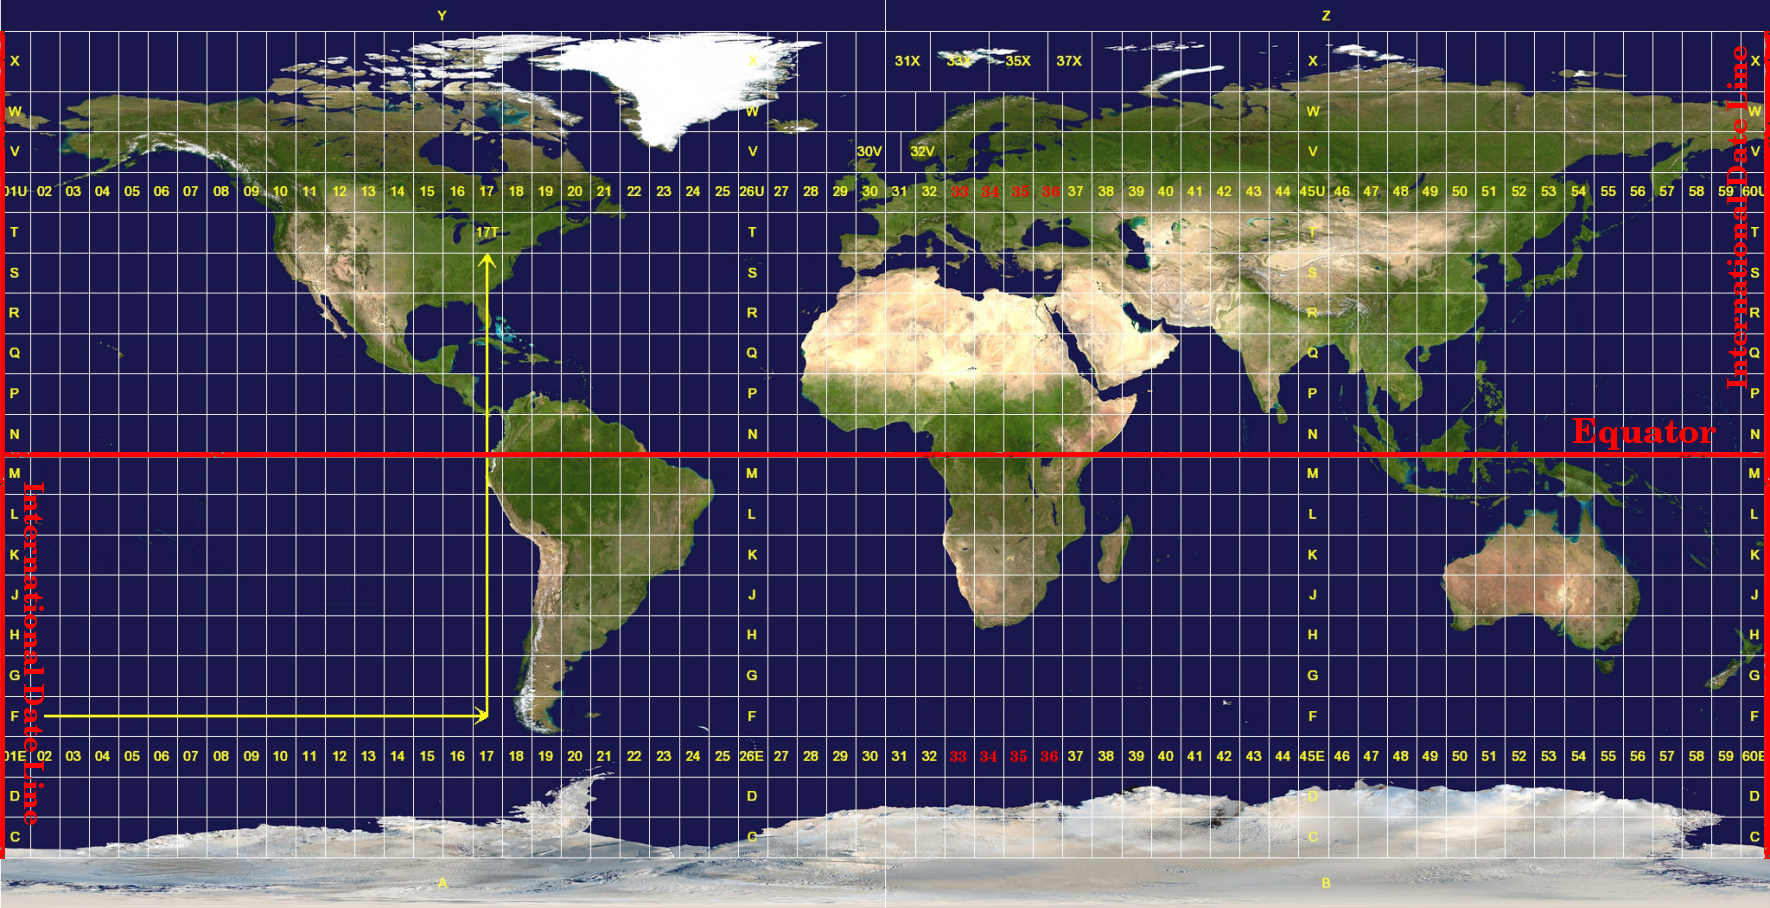
\includegraphics[width=0.75\linewidth]{images/spatial_data_viz/utm_zones} 

}

\caption{UTM Zones of the world}\label{fig:unnamed-chunk-4}
\end{figure}

\newpage

\hypertarget{introduction-to-qgis}{%
\section{Introduction to QGIS}\label{introduction-to-qgis}}

\href{https://qgis.org/}{QGIS} is a free and open-source software for
creating, editing, visualizing, analyzing and publishing geospatial
data. QGIS is available for Windows, Mac and Linux. This class uses QGIS
for the exercises.

Visit the
\href{https://qgis.org/en/site/forusers/download.html}{download page} to
download and install the latest LTR (Long Term Release) stable version.

\hypertarget{plugins}{%
\subsection{Plugins}\label{plugins}}

QGIS offers an easy way for developers to extend the core functionality
of the software using plugins. Plugins can be installed from QGIS from
\textbf{Plugins → Manage and Install Plugins..}. To install a plugin,
switch to the \emph{All} tab and search for the plugin. Once you find
it, select and click \emph{Install Plugin}.

\begin{center}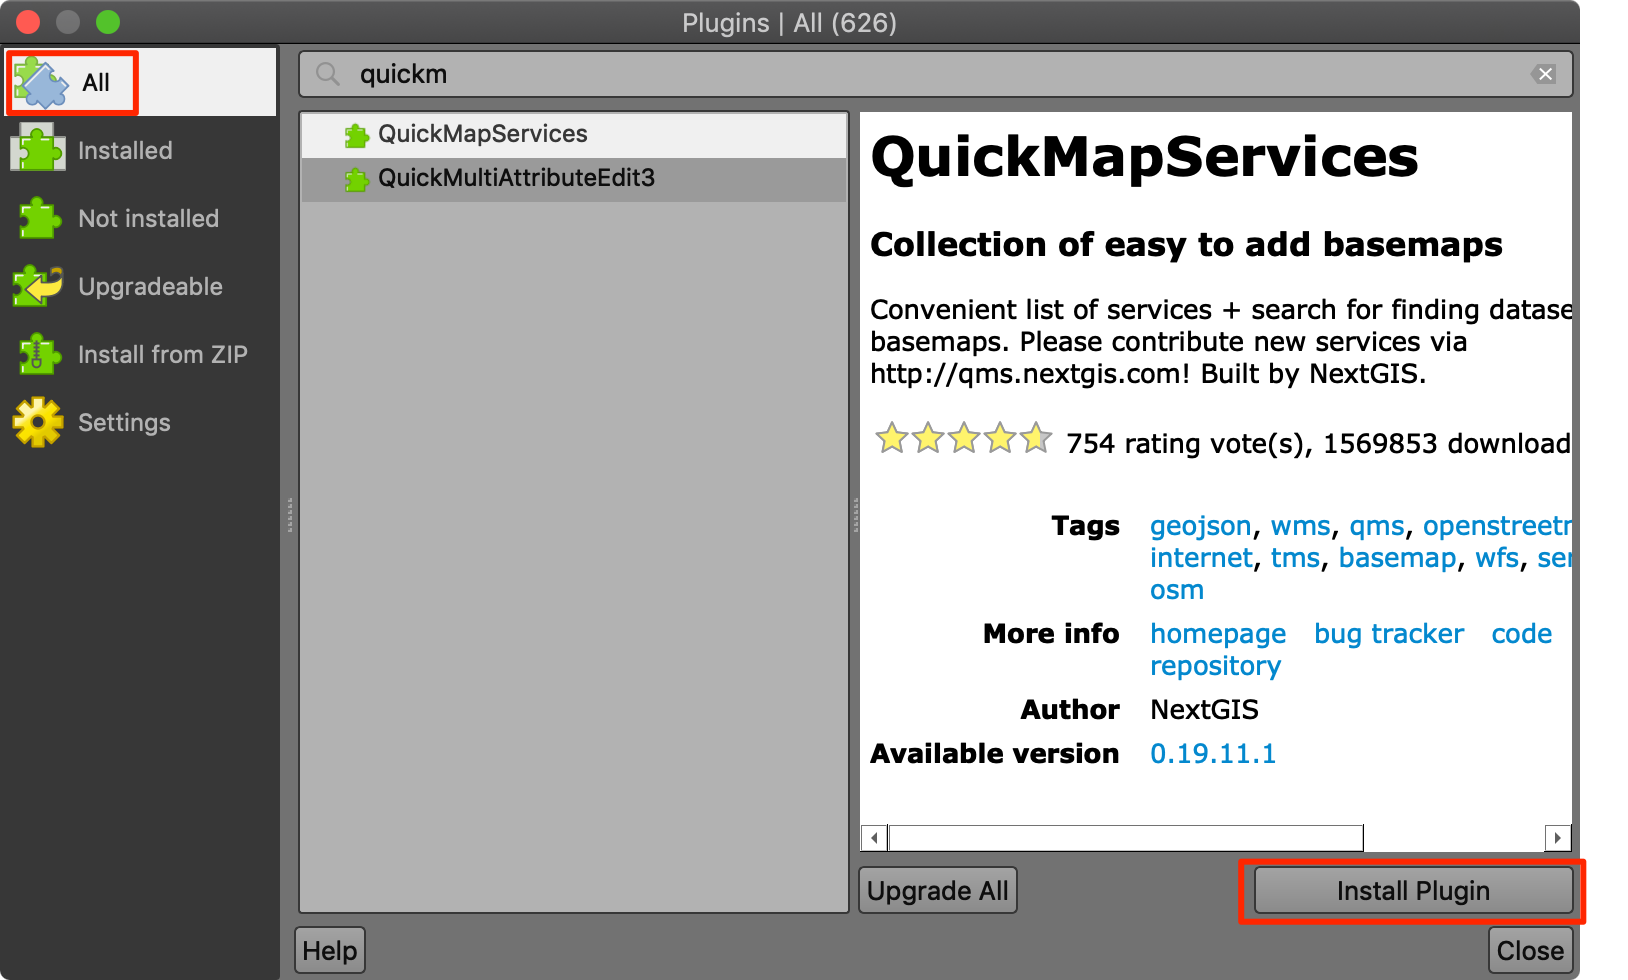
\includegraphics[width=0.75\linewidth]{images/spatial_data_viz/plugins} \end{center}

For this class, we will be using the following plugins. Go ahead and
install them.

\begin{itemize}
\tightlist
\item
  QuickMapServices
\item
  TimeManager
\item
  QuickOSM
\end{itemize}

\newpage

\hypertarget{visualization}{%
\section{Visualization}\label{visualization}}

\hypertarget{points}{%
\subsection{Points}\label{points}}

The simplest representation of spatial data can be done using a table. A
place can be represented using a pair of coordinates - Latitude and
Longitude - with other attribute information about the place. Many
spatial data source come in this form. Excel sheets, CSV files, database
tables etc.

\hypertarget{exercise-mapping-air-quality}{%
\subsubsection{Exercise: Mapping Air
Quality}\label{exercise-mapping-air-quality}}

Worsening air quality is a severe problem in many countries around the
world. India - particularly - Delhi suffers from
\href{https://ig.ft.com/india-pollution/}{acute problems of high
pollution levels}.One of the first steps to better understand the
problem, is to have continuous monitoring of air quality across the
cities. Many organizations have stepped up and setup such sensors that
collect air quality data and make it publicly available.
\href{https://openaq.org/}{OpenAQ} is a platform that collects this data
from all public sources and makes it available in an easy to use form.

\begin{quote}
\begin{quote}
If you are interested in this air quality in India,
\href{http://www.urbanemissions.info/}{Urban Emissions} has a lot of
relevant information and datasets.
\end{quote}
\end{quote}

We will take the sensor data for
\href{https://blissair.com/what-is-pm-2-5.htm}{PM2.5 concentrations} 1
day and map it. The aim is to turn this tabular data info an informative
spatial data visualization.

For this exercise, we are using daily average data for Delhi, India for
February 15, 2020. This data was downloaded from
\href{https://openaq.org/\#/countries?_k=dmlk2k}{OpenAQ Data Download}

\begin{center}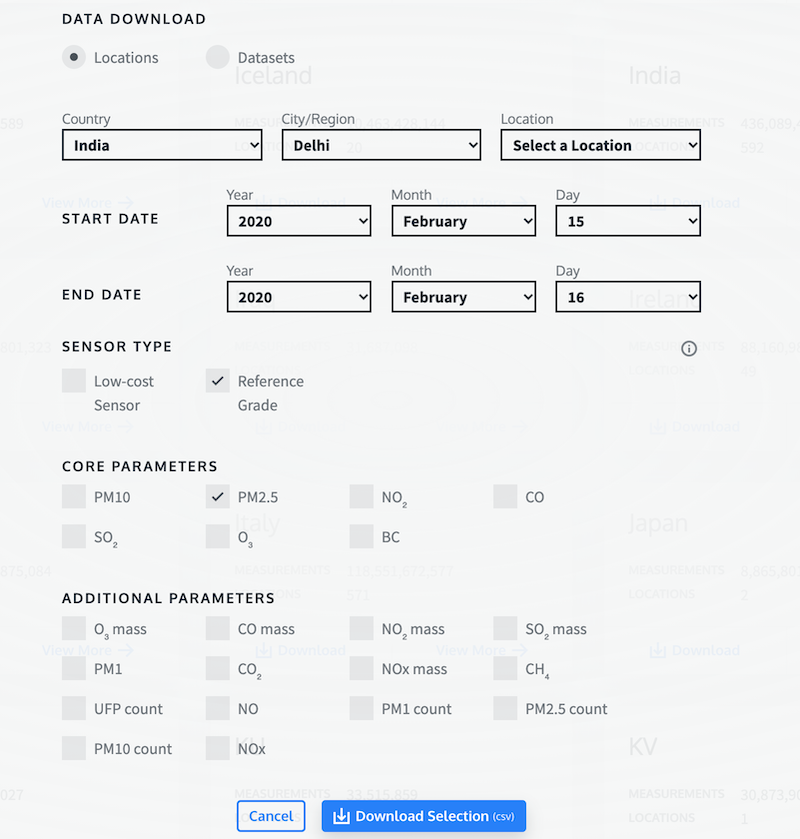
\includegraphics[width=0.75\linewidth]{images/spatial_data_viz/aq0} \end{center}

\begin{enumerate}
\def\labelenumi{\arabic{enumi}.}
\tightlist
\item
  Open the \texttt{openaq.csv} file in a text editor and examine it.
  Each row of data contains data from 1 monitoring station. The
  \texttt{latitude} and \texttt{longitude} column contain the
  coordinates of the station and the \texttt{value} contains the daily
  average PM2.5 concentration
\end{enumerate}

\begin{center}\includegraphics[width=0.75\linewidth]{images/spatial_data_viz/aq1} \end{center}

\begin{enumerate}
\def\labelenumi{\arabic{enumi}.}
\setcounter{enumi}{1}
\tightlist
\item
  Tabular data in text files fall into the category of \textbf{Delimited
  Text} files, such as this can be imported in QGIS via \emph{Data
  Source Manager}. Click \emph{Open Data Source Manager} button.
\end{enumerate}

\begin{center}\includegraphics[width=0.75\linewidth]{images/spatial_data_viz/aq2} \end{center}

\begin{enumerate}
\def\labelenumi{\arabic{enumi}.}
\setcounter{enumi}{2}
\tightlist
\item
  Browse to the \texttt{openaq.csv} file and open it. As we want to
  import this file as points, select \emph{Point coordinates}. Choose
  \texttt{longitude} as \emph{X Field} and \texttt{latitude} as \emph{Y
  Field}. Choose \texttt{EPSG\ 4326\ -\ WGS\ 84} in \emph{Geometry CRS}.
  Click \emph{Add}.
\end{enumerate}

\begin{center}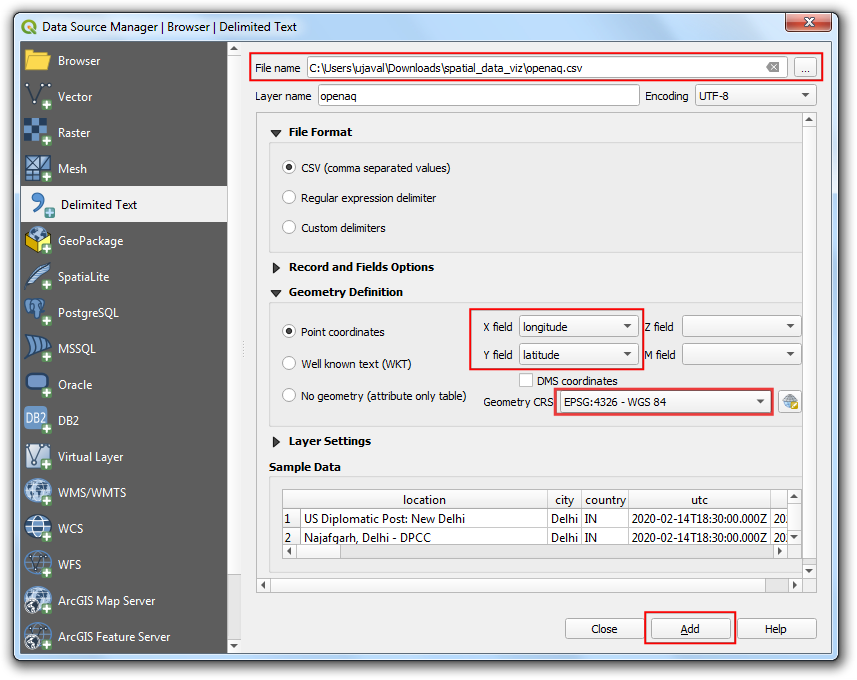
\includegraphics[width=0.75\linewidth]{images/spatial_data_viz/aq3} \end{center}

\begin{enumerate}
\def\labelenumi{\arabic{enumi}.}
\setcounter{enumi}{3}
\tightlist
\item
  You will see the tabular data now loaded in QGIS canvas as a spatial
  data layer. Use the \emph{Identify} button and click on any of the
  point. You will see the attribute data that is attached to each point.
\end{enumerate}

\begin{center}\includegraphics[width=0.75\linewidth]{images/spatial_data_viz/aq4} \end{center}

\begin{quote}
Note: If you don't see the OpenStreetMap monochrome, Go to \textbf{Web →
QuickMapServices → Settings}, switch to \textbf{More servises}, click
\texttt{Get\ Contributed\ Pack}. Click \textbf{Save}.
\end{quote}

\begin{center}\includegraphics[width=0.75\linewidth]{images/spatial_data_viz/aq5} \end{center}

\begin{enumerate}
\def\labelenumi{\arabic{enumi}.}
\setcounter{enumi}{5}
\tightlist
\item
  A new layer will get added to the \emph{Layers} panel and the
  \emph{Canvas}. Now you can see the points in the context of the city
  and surroundings. Let's style the point layer better now. Click
  \emph{Open the Layer Styling Panel}.
\end{enumerate}

\begin{center}\includegraphics[width=0.75\linewidth]{images/spatial_data_viz/aq6} \end{center}

\begin{enumerate}
\def\labelenumi{\arabic{enumi}.}
\setcounter{enumi}{6}
\tightlist
\item
  We will color each point according to the observed PM2.5 value. Choose
  \texttt{Graduated} renderer and \texttt{value} as the \emph{Value}
  column. Set the number of \emph{Classes} to \texttt{6} and click
  \emph{Classify}.
\end{enumerate}

\begin{center}\includegraphics[width=0.75\linewidth]{images/spatial_data_viz/aq7} \end{center}

For the class ranges to have some meaning, we need to link them to the
commonly used scale. India has adopted
\href{https://pib.gov.in/newsite/PrintRelease.aspx?relid=110654}{National
Air Quality Index} with the following definitions.

\begin{center}\includegraphics[width=0.75\linewidth]{images/spatial_data_viz/aq_naqi} \end{center}

\begin{enumerate}
\def\labelenumi{\arabic{enumi}.}
\setcounter{enumi}{7}
\tightlist
\item
  Let's adjust the class values to match those defined in the National
  Air Quality Index. We can also change the \emph{Legend} labels to the
  human-readable category names. You can double-click each class range
  and edit it.
\end{enumerate}

\begin{quote}
Note: The range boundaries includes the upper bound value but excludes
the lower bound value. So if the range is 30-60, the range will include
all values \textgreater30 and \textless=60. See the
\href{https://github.com/qgis/QGIS/issues/29852}{discussion here} for
more info.
\end{quote}

\begin{center}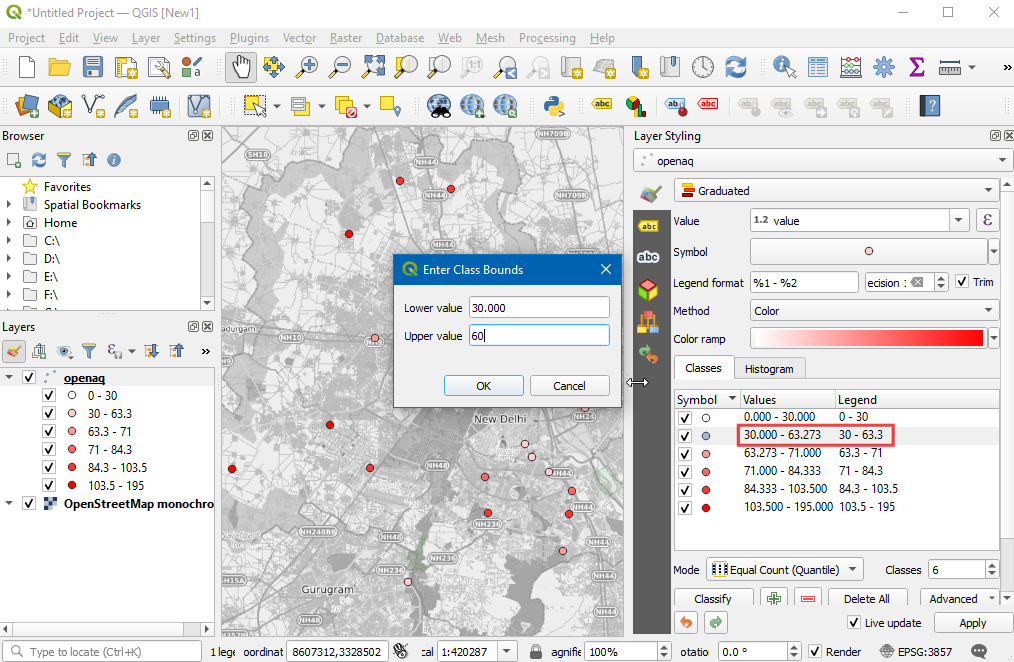
\includegraphics[width=0.75\linewidth]{images/spatial_data_viz/aq8} \end{center}

\begin{enumerate}
\def\labelenumi{\arabic{enumi}.}
\setcounter{enumi}{8}
\tightlist
\item
  As you edit the categories, the map visualization will change
  accordingly. The layer legend will also show the legend labels now.
\end{enumerate}

\begin{center}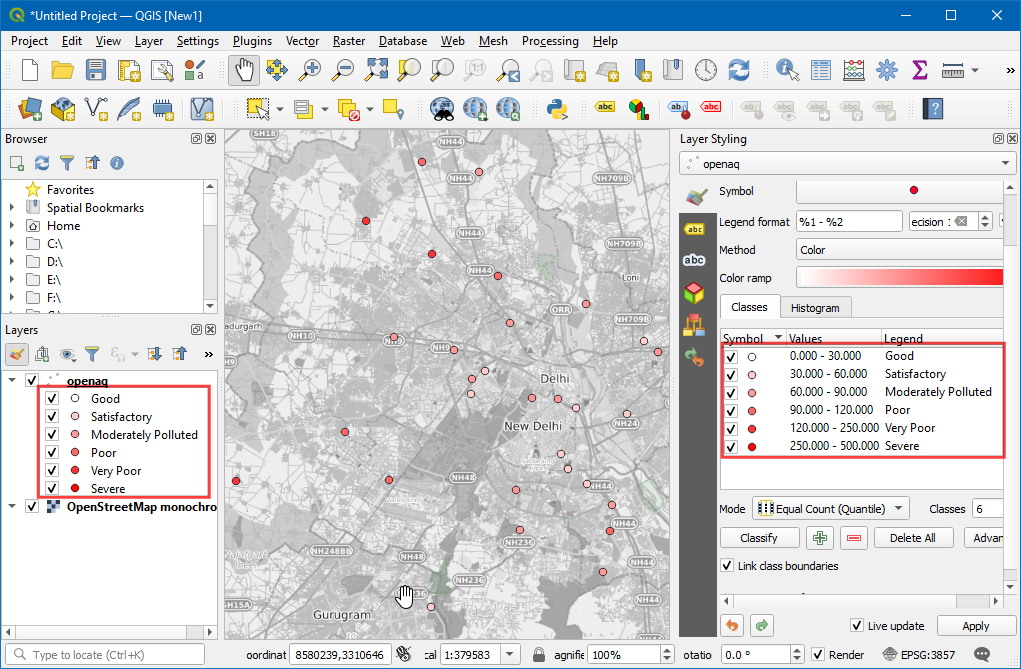
\includegraphics[width=0.75\linewidth]{images/spatial_data_viz/aq9} \end{center}

\begin{enumerate}
\def\labelenumi{\arabic{enumi}.}
\setcounter{enumi}{9}
\tightlist
\item
  We can change the color also to match those defined in the index.
  Select the dropdown next to the color ramp and select the
  \texttt{RdYlGn} (Red-Yellow-Green) ramp.
\end{enumerate}

\begin{center}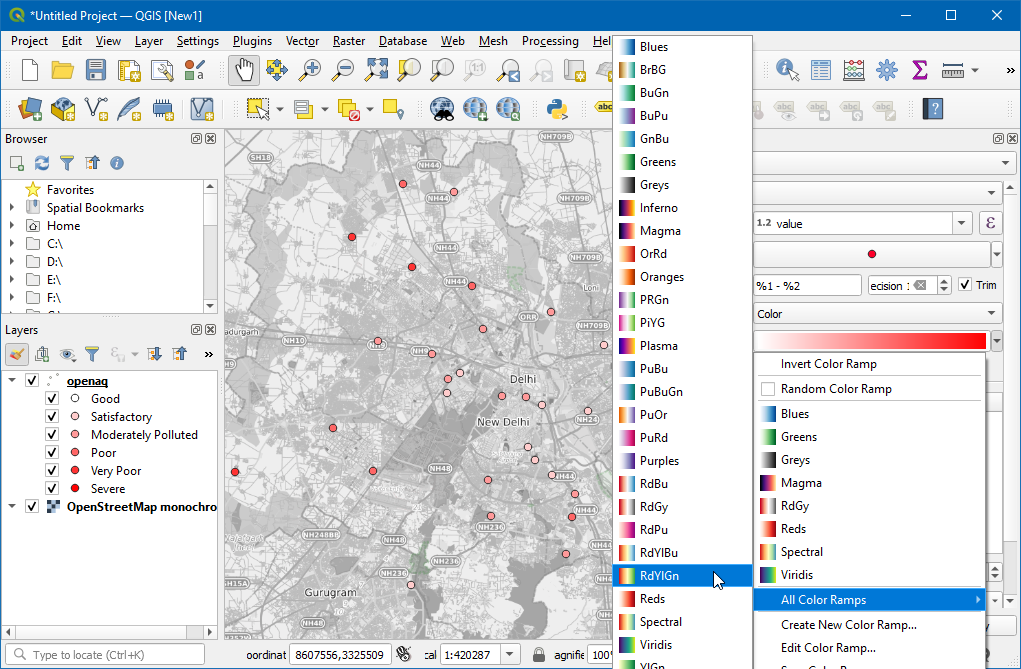
\includegraphics[width=0.75\linewidth]{images/spatial_data_viz/aq10} \end{center}

\begin{enumerate}
\def\labelenumi{\arabic{enumi}.}
\setcounter{enumi}{10}
\tightlist
\item
  We want the ramp to go from Green (low PM2.5 values) to Red (high
  PM2.5 values) - so click the dropdown again and select \emph{Invert
  Color Ramp}.
\end{enumerate}

\begin{center}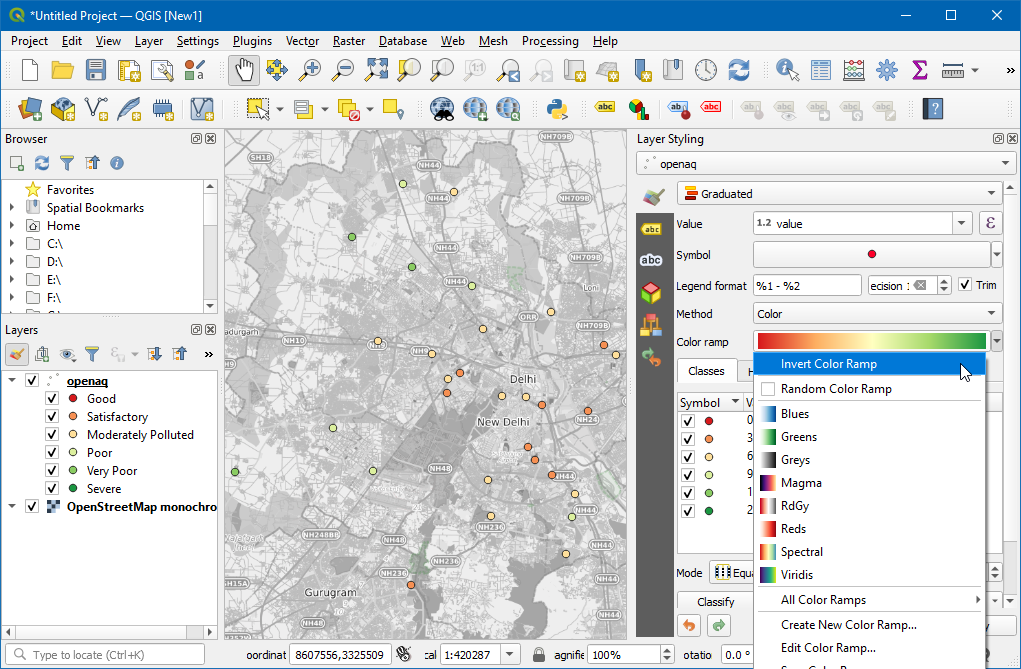
\includegraphics[width=0.75\linewidth]{images/spatial_data_viz/aq11} \end{center}

\begin{enumerate}
\def\labelenumi{\arabic{enumi}.}
\setcounter{enumi}{11}
\tightlist
\item
  We will add labels to the points now. Switch to the \emph{Labels} tab.
\end{enumerate}

\begin{center}\includegraphics[width=0.75\linewidth]{images/spatial_data_viz/aq12} \end{center}

\begin{enumerate}
\def\labelenumi{\arabic{enumi}.}
\setcounter{enumi}{12}
\tightlist
\item
  Choose \texttt{Single\ labels} and \texttt{value} as \emph{Value}.
  Scroll down and check \emph{Formatted numbers} and change the
  \emph{Decimal places} to \texttt{0}.
\end{enumerate}

\begin{center}\includegraphics[width=0.75\linewidth]{images/spatial_data_viz/aq13} \end{center}

\begin{enumerate}
\def\labelenumi{\arabic{enumi}.}
\setcounter{enumi}{13}
\tightlist
\item
  Next, switch to the \emph{Background} tab. Check \emph{Draw
  background} and adjust the \emph{Size X} and \emph{Size Y}.
\end{enumerate}

\begin{center}\includegraphics[width=0.75\linewidth]{images/spatial_data_viz/aq14} \end{center}

\begin{enumerate}
\def\labelenumi{\arabic{enumi}.}
\setcounter{enumi}{14}
\tightlist
\item
  Scroll down to the \emph{Fill color} section. We want the fill color
  for each box to match the color of the associated point. Click the
  \emph{Data defined override} button and choose \emph{Edit}.
\end{enumerate}

\begin{center}\includegraphics[width=0.75\linewidth]{images/spatial_data_viz/aq15} \end{center}

\begin{enumerate}
\def\labelenumi{\arabic{enumi}.}
\setcounter{enumi}{15}
\tightlist
\item
  Double-click the \texttt{@symbol\_color} variable to add it to the
  expression. Click OK.
\end{enumerate}

\begin{center}\includegraphics[width=0.75\linewidth]{images/spatial_data_viz/aq16} \end{center}

\begin{enumerate}
\def\labelenumi{\arabic{enumi}.}
\setcounter{enumi}{16}
\tightlist
\item
  You will see the map change and the label shields will have the color
  matching the category based on the values. We will move the labels
  slightly above so the points are also seen. Switch to the
  \emph{Placement} tab and select \emph{Offset from point}. Check the
  \emph{Offset Y} to \texttt{-5}.
\end{enumerate}

\begin{center}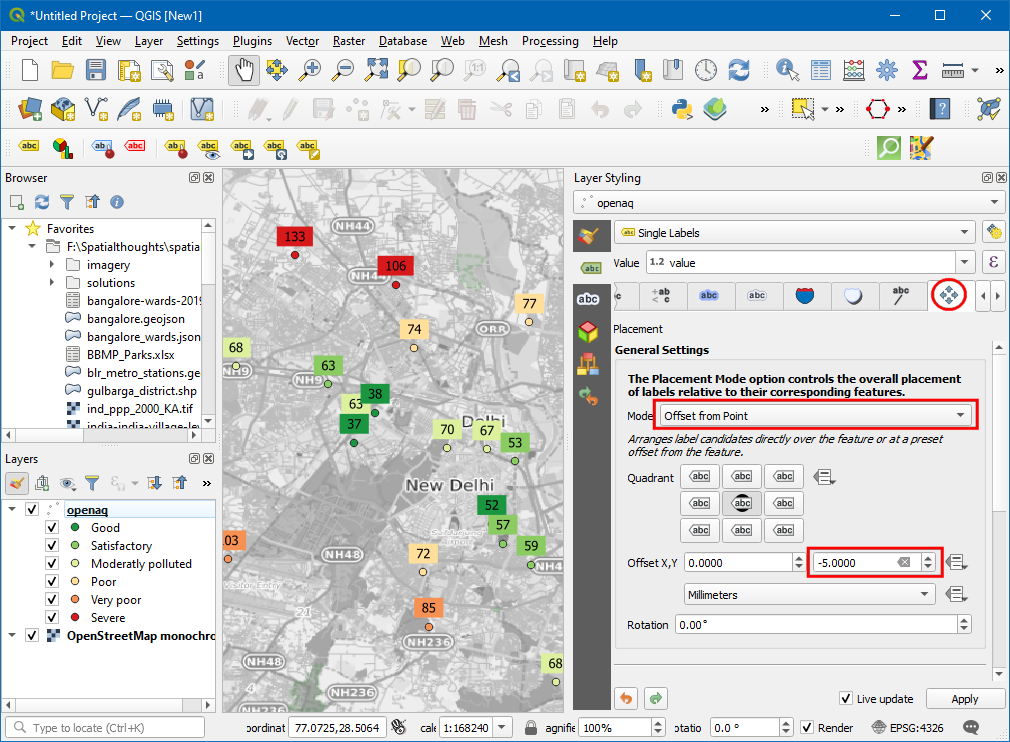
\includegraphics[width=0.75\linewidth]{images/spatial_data_viz/aq17} \end{center}

\begin{enumerate}
\def\labelenumi{\arabic{enumi}.}
\setcounter{enumi}{17}
\tightlist
\item
  Lastly, go the \emph{Callouts} tab and check \emph{Draw callouts} to
  make it easy to see which labels belong to which point.
\end{enumerate}

\begin{center}\includegraphics[width=0.75\linewidth]{images/spatial_data_viz/aq18} \end{center}

\begin{enumerate}
\def\labelenumi{\arabic{enumi}.}
\setcounter{enumi}{18}
\tightlist
\item
  It is a good idea to save out work. Click the \emph{Save Project}
  button and save it as \texttt{air\_quality.qgz}.
\end{enumerate}

\begin{center}\includegraphics[width=0.75\linewidth]{images/spatial_data_viz/aq19} \end{center}

\begin{enumerate}
\def\labelenumi{\arabic{enumi}.}
\setcounter{enumi}{19}
\tightlist
\item
  You can see most of the labels are legible, but some are too close and
  feel a bit cluttered. We can fix them by manually adjusting the
  placement. Right-click anywhere on the toolbar area and enable the
  \emph{Label Toolbar}.
\end{enumerate}

\begin{center}\includegraphics[width=0.75\linewidth]{images/spatial_data_viz/aq20} \end{center}

\begin{enumerate}
\def\labelenumi{\arabic{enumi}.}
\setcounter{enumi}{20}
\tightlist
\item
  Click the \emph{Move a Label} button. Click \emph{OK} on the
  \emph{Auxiliary Storage} prompt.
\end{enumerate}

\begin{center}\includegraphics[width=0.75\linewidth]{images/spatial_data_viz/aq21} \end{center}

\begin{enumerate}
\def\labelenumi{\arabic{enumi}.}
\setcounter{enumi}{21}
\tightlist
\item
  With the \emph{Move a Label} button active, click on a any label to
  select it. Click at the place you want to move it to, and it will be
  placed there. Once you are satisfied, save the project. It is time to
  export our map. Go to \textbf{Project → New Print Layout\ldots{}}.
  Leave the name empty and click \emph{OK}.
\end{enumerate}

\begin{center}\includegraphics[width=0.75\linewidth]{images/spatial_data_viz/aq22} \end{center}

\begin{enumerate}
\def\labelenumi{\arabic{enumi}.}
\setcounter{enumi}{22}
\tightlist
\item
  Print Layouts are a way to compose a static map with various elements
  such as labels, legends, north arrow, scale bar etc. Go to \textbf{Add
  Item → Add Map}.
\end{enumerate}

\begin{center}\includegraphics[width=0.75\linewidth]{images/spatial_data_viz/aq23} \end{center}

\begin{enumerate}
\def\labelenumi{\arabic{enumi}.}
\setcounter{enumi}{23}
\tightlist
\item
  Drag a rectangle where you want the map to be rendered. Once you let
  go of you your mouse button, the map from the main canvas will be
  loaded in the region.
\end{enumerate}

\begin{quote}
If you do not see the full extent of your map in the region, you can
click the \emph{Set Map Extent to Match Main Canvas Extent} button
located in the toolbar under \emph{Item Properties} for \texttt{Map\ 1}
\end{quote}

\begin{center}\includegraphics[width=0.75\linewidth]{images/spatial_data_viz/aq24} \end{center}

\begin{enumerate}
\def\labelenumi{\arabic{enumi}.}
\setcounter{enumi}{24}
\tightlist
\item
  Next, we will add a \emph{Rectangle} which will hold the tile, legend
  and attribution.
\end{enumerate}

\begin{center}\includegraphics[width=0.75\linewidth]{images/spatial_data_viz/aq25} \end{center}

\begin{enumerate}
\def\labelenumi{\arabic{enumi}.}
\setcounter{enumi}{25}
\tightlist
\item
  Place the rectangle on the top-right hand corner and change the
  \emph{Corner radius} to \texttt{10}.
\end{enumerate}

\begin{center}\includegraphics[width=0.75\linewidth]{images/spatial_data_viz/aq26} \end{center}

\begin{enumerate}
\def\labelenumi{\arabic{enumi}.}
\setcounter{enumi}{26}
\tightlist
\item
  Next, add a \emph{Label} within the rectangle we just created. Enter
  the title \texttt{Average\ PM2.5\ Concentration\ (µg/m3)} and date
  \texttt{15\ February,\ 2020}.
\end{enumerate}

\begin{center}\includegraphics[width=0.75\linewidth]{images/spatial_data_viz/aq27} \end{center}

\begin{enumerate}
\def\labelenumi{\arabic{enumi}.}
\setcounter{enumi}{27}
\tightlist
\item
  In the same rectangle, add another \emph{Label} with the attribution
  text
  \texttt{Data\ Source:\ Central\ Pollution\ Control\ Board,\ EPA\ AirNow\ DOS.\ Downloaded\ from\ OpenAQ.org}.
  Now we will add a legend, so our users know how to interpret various
  colors on the map. Go to \textbf{Add Item → Add Legend}
\end{enumerate}

\begin{center}\includegraphics[width=0.75\linewidth]{images/spatial_data_viz/aq28} \end{center}

\begin{enumerate}
\def\labelenumi{\arabic{enumi}.}
\setcounter{enumi}{28}
\tightlist
\item
  Drag a box to insert the legend in the rectangle. Go to the \emph{Item
  Properties} tab and turn-off \emph{Auto update}. Remove the
  \texttt{OpenStreetMap\ monochrome} layer and set the \texttt{openaq}
  group label to \emph{Hidden}.
\end{enumerate}

\begin{center}\includegraphics[width=0.75\linewidth]{images/spatial_data_viz/aq29} \end{center}

\begin{enumerate}
\def\labelenumi{\arabic{enumi}.}
\setcounter{enumi}{29}
\tightlist
\item
  The default legend placement is vertical - in a single column. We can
  change it to be in multiple columns to make it span horizontal. Scroll
  down to the \emph{Columns} section and change the \emph{Count} to
  \texttt{2} and check \emph{Split layers} button.
\end{enumerate}

\begin{center}\includegraphics[width=0.75\linewidth]{images/spatial_data_viz/aq30} \end{center}

\begin{enumerate}
\def\labelenumi{\arabic{enumi}.}
\setcounter{enumi}{30}
\tightlist
\item
  In the \emph{Main Properties} section, enter a \emph{Title} for the
  legend as \texttt{Air\ Quality\ Index\ Category}.
\end{enumerate}

\begin{center}\includegraphics[width=0.75\linewidth]{images/spatial_data_viz/aq31} \end{center}

\begin{enumerate}
\def\labelenumi{\arabic{enumi}.}
\setcounter{enumi}{31}
\tightlist
\item
  Once you are satisfied with the map, we can export the map. You can
  export the composition as an \textbf{Image} if you wanted to use it in
  a website, email, slideshow etc. You can also export it to as an
  \textbf{SVG} so it can be further edited in a graphics program such as
  \href{https://inkscape.org/}{InkScape}. But the most common format for
  maps is still a PDF.
\end{enumerate}

\begin{figure}

{\centering \includegraphics[width=0.75\linewidth]{images/spatial_data_viz/shp_to_pdf} 

}

\caption{Credit: Atanas Entchev}\label{fig:unnamed-chunk-39}
\end{figure}

So let's export our map to a PDF. Before exporting, switch to the
\emph{Layout} tab. We are using the basemap layer from OpenStreetMap.
This layer is created using individual tiles that are zoom dependent.
Setting a higher export resolution will fetch higher resolution tiles
with different labeling scheme when exporting. You may experiment with
this value to get the right level of detail in the basemap. For this
particular exercise \emph{Export resolution} to \texttt{100} dpi works
well. Go to \textbf{Layout → Export as PDF}.

\begin{center}\includegraphics[width=0.75\linewidth]{images/spatial_data_viz/aq32} \end{center}

\begin{enumerate}
\def\labelenumi{\arabic{enumi}.}
\setcounter{enumi}{32}
\tightlist
\item
  In the \emph{PDF Export Options}, you can check \emph{Create
  Geospatial PDF (GeoPDF)}. GeoPDF is an enhanced PDF format that is
  spatially aware and preserves layer and attribute information. Click
  \emph{Save} and save the output as \texttt{delhi\_air\_quality.pdf}.
\end{enumerate}

\begin{center}\includegraphics[width=0.75\linewidth]{images/spatial_data_viz/aq33} \end{center}

\begin{enumerate}
\def\labelenumi{\arabic{enumi}.}
\setcounter{enumi}{33}
\tightlist
\item
  If you open the resulting PDF in a compatible reader such as
  \href{https://get.adobe.com/reader/}{Adobe Acrobat}, you can toggle
  layer visibility, query attributes by features, measure distances and
  so on.
\end{enumerate}

\begin{quote}
In Adobe Reader, you can enable the measuring tool by going to Tools →
Measure.
\href{https://helpx.adobe.com/in/acrobat/using/grids-guides-measurements-pdfs.html\#measure_the_height_width_or_area_of_objects}{Learn
more}
\end{quote}

\begin{center}\includegraphics[width=0.75\linewidth]{images/spatial_data_viz/aq34} \end{center}

\newpage

\hypertarget{lines}{%
\subsection{Lines}\label{lines}}

Many of our transportation infrastructure such as roads, bridges,
railways etc. as well as natural features such as rivers, streams etc.
can be modeled as lines. Other abstract concepts, such as contours and
trajectories are also modeled using linear features. Shapefiles,
GeoJSON, GPX are commonly used file formats for storing line datasets.

\hypertarget{exercise-visualize-gps-tracks}{%
\subsubsection{Exercise: Visualize GPS
Tracks}\label{exercise-visualize-gps-tracks}}

GPS tracks have become ubiquitous in modern life. With GPS built-into
most phones, many of us capture the tracks while running or biking
outdoors. Cab companies use GPS tracks collected during the trip to
determine fares. Delivery and logistics companies store and analyze
millions of GPS tracks from their assets to derive location
intelligence.

We will use a GPS track I collected using the open-source
\href{https://www.basicairdata.eu/projects/android/android-gps-logger/}{GPS
Logger app} while cycling to work. The default format for storing GPS
tracks is \href{https://en.wikipedia.org/wiki/GPS_Exchange_Format}{GPS
Exchange Format (GPX)}. It is a XML-based text format that allows
storing points, tracks and routes in a single file. We will use the data
in \texttt{sample\_gps\_track.gpx} file and create an animated GIF
showing the trip.

\begin{enumerate}
\def\labelenumi{\arabic{enumi}.}
\tightlist
\item
  Locate the \texttt{sample\_gps\_track.gpx} file and drag it to the
  canvas.
\end{enumerate}

\begin{center}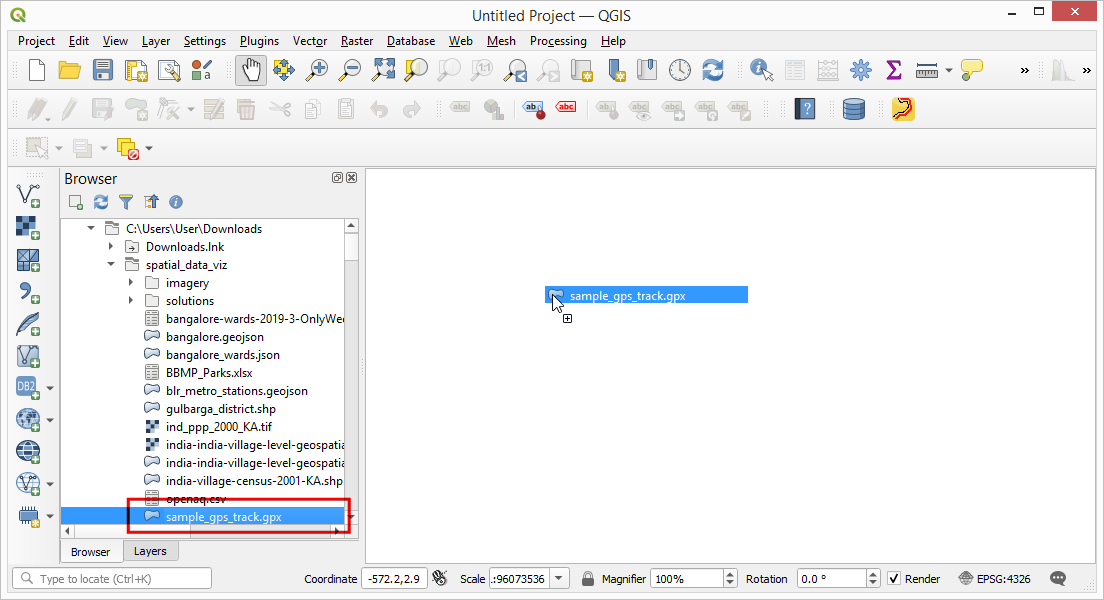
\includegraphics[width=0.75\linewidth]{images/spatial_data_viz/gps1} \end{center}

\begin{enumerate}
\def\labelenumi{\arabic{enumi}.}
\setcounter{enumi}{1}
\tightlist
\item
  As the file contains multiple data types, a pop-up will ask us to
  select the layers to add. Hold the \emph{Shift} key and select both
  \texttt{track\_points} and \texttt{tracks} layers. Click \emph{OK}.
\end{enumerate}

\begin{center}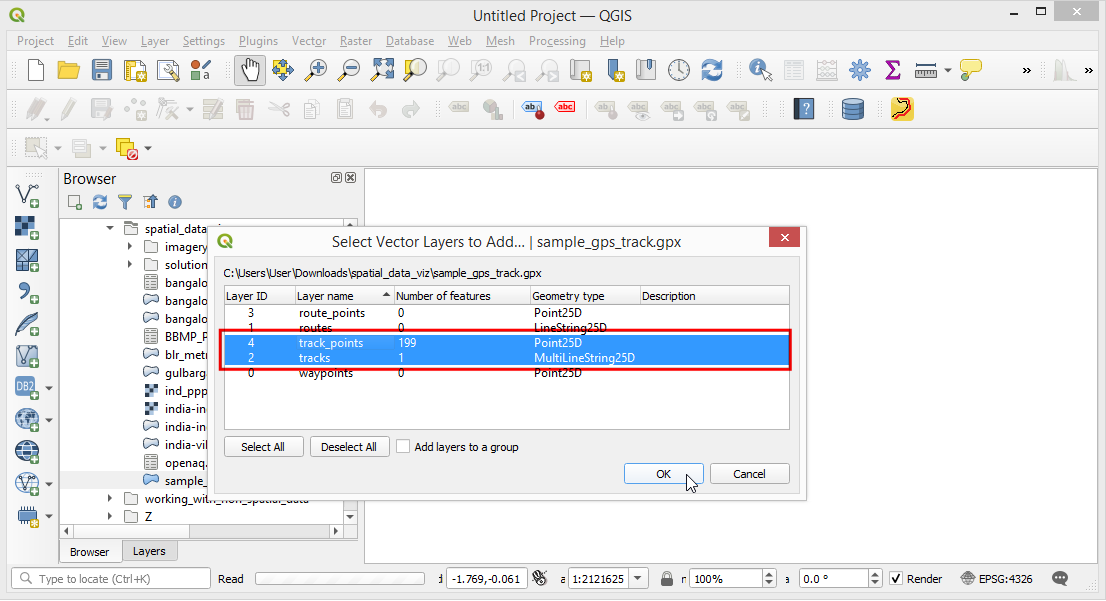
\includegraphics[width=0.75\linewidth]{images/spatial_data_viz/gps2} \end{center}

\begin{enumerate}
\def\labelenumi{\arabic{enumi}.}
\setcounter{enumi}{2}
\tightlist
\item
  To add some context to the map, we should add a basemap. A dark
  background map works best for the visualization we want to create. Go
  to \textbf{Web → QuickMapServices → CartoDB → Dark Matter} layer.
\end{enumerate}

\begin{center}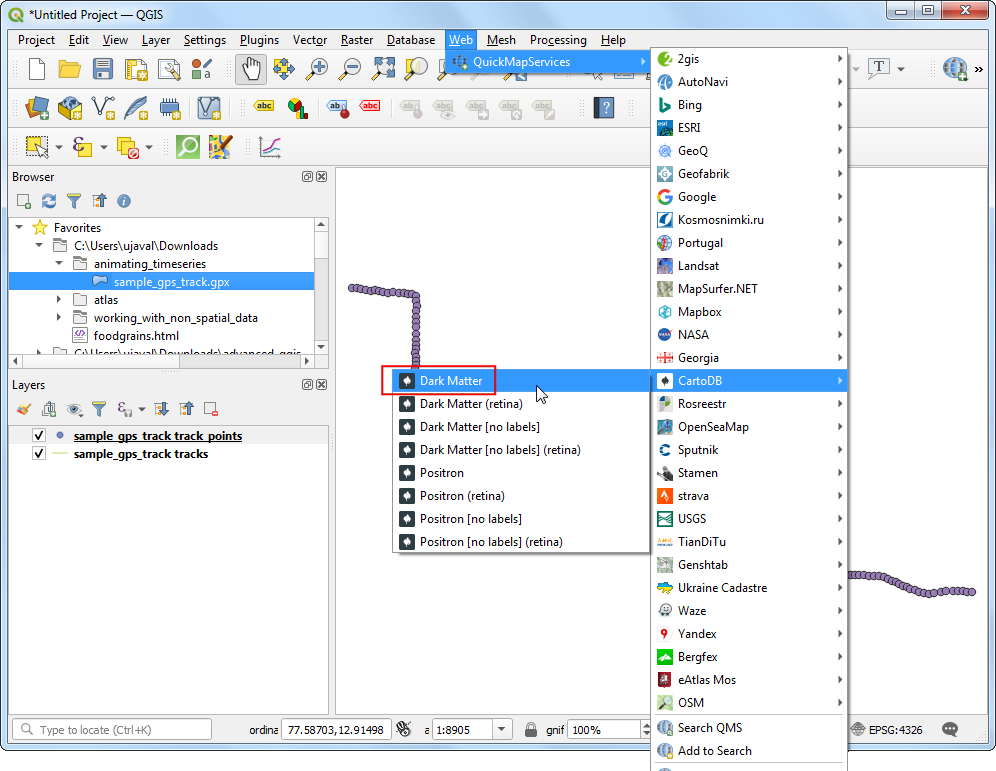
\includegraphics[width=0.75\linewidth]{images/spatial_data_viz/gps3} \end{center}

\begin{enumerate}
\def\labelenumi{\arabic{enumi}.}
\setcounter{enumi}{3}
\tightlist
\item
  Turn off the visibility of the \texttt{sample\_gps\_track\ points}
  layer by un-checking the box next to it. Select the
  \texttt{sample\_gps\_track\ tracks} layer and click \emph{Open the
  Layer Styling Panel}. You can change the line \emph{Color} to
  \texttt{Blue} and \emph{Width} to \texttt{0.5}.
\end{enumerate}

\begin{center}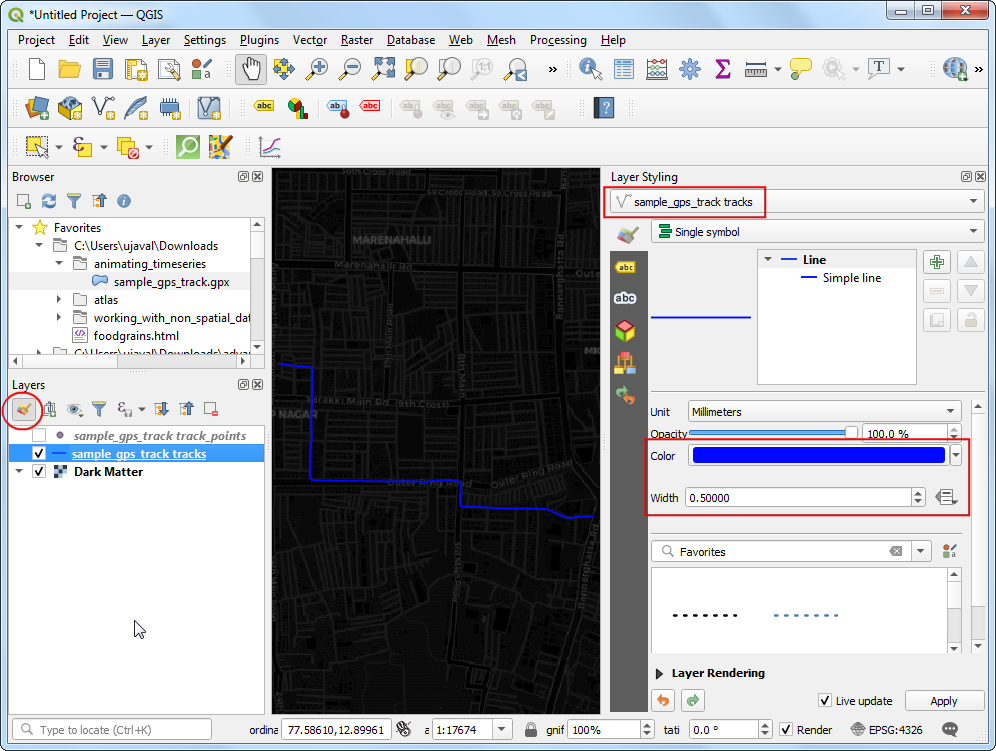
\includegraphics[width=0.75\linewidth]{images/spatial_data_viz/gps4} \end{center}

\begin{enumerate}
\def\labelenumi{\arabic{enumi}.}
\setcounter{enumi}{4}
\tightlist
\item
  Turn on the visibility of the \texttt{sample\_gps\_track\ points}
  layer and select it. In the \emph{Layer Styling Panel}, select
  \emph{Simple marker} symbol. Change the point \emph{Size} to
  \texttt{1} . Choose a lighter shade of Blue as the \emph{Fill color}
  and a \texttt{Transparent\ Stroke} as \emph{Stroke color}.
\end{enumerate}

\begin{center}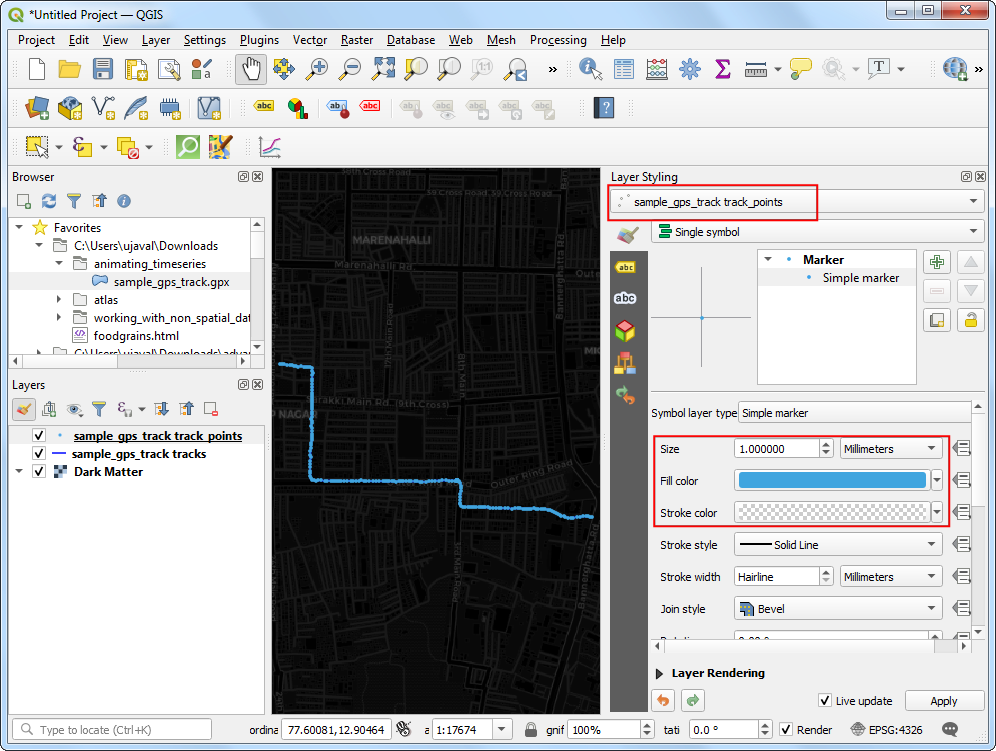
\includegraphics[width=0.75\linewidth]{images/spatial_data_viz/gps5} \end{center}

\begin{enumerate}
\def\labelenumi{\arabic{enumi}.}
\setcounter{enumi}{5}
\tightlist
\item
  We want to give a glow effect to the points as it is animating.
  Right-click the \texttt{gps\_points} layer and choose \emph{Duplicate
  Layer}.
\end{enumerate}

\begin{center}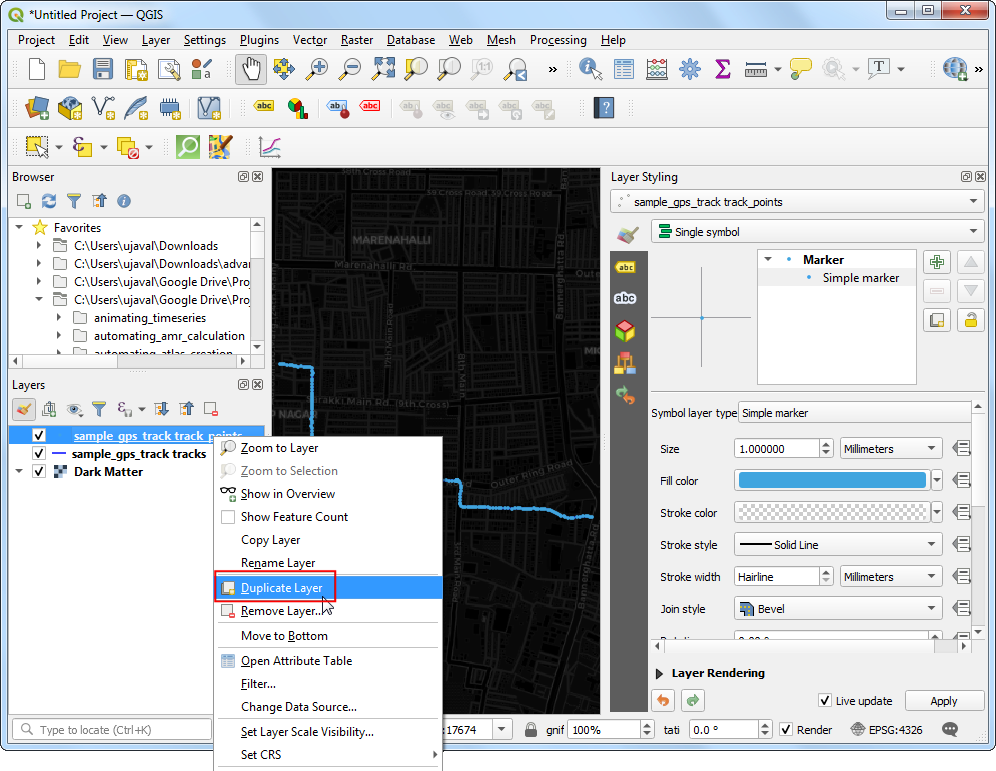
\includegraphics[width=0.75\linewidth]{images/spatial_data_viz/gps6} \end{center}

\begin{enumerate}
\def\labelenumi{\arabic{enumi}.}
\setcounter{enumi}{6}
\tightlist
\item
  Drag the duplicate layer on top of the stack in the \emph{Layers}
  panel. In the \emph{Layer Styling Panel} for the duplicated
  \texttt{sample\_gps\_track\ points\_copy} layer, choose bright neon as
  the \emph{Color} from the color picker and increase the size to
  \texttt{1.5}. Check the \emph{Draw Effects} option and click the
  \emph{Effects} button next to it.
\end{enumerate}

\begin{center}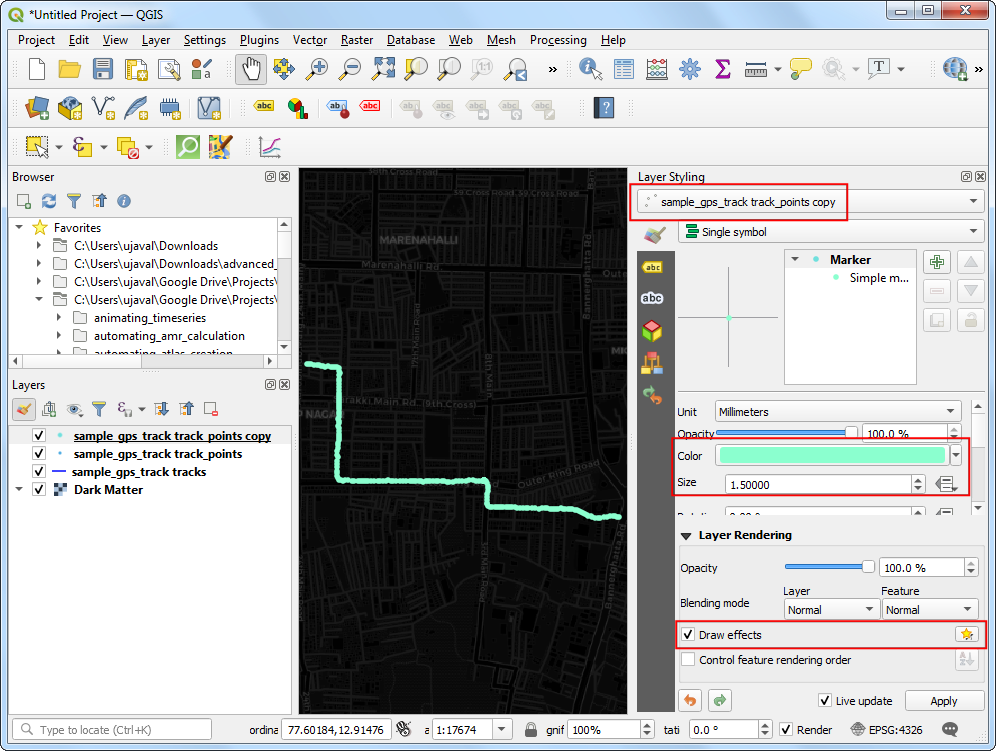
\includegraphics[width=0.75\linewidth]{images/spatial_data_viz/gps7} \end{center}

\begin{enumerate}
\def\labelenumi{\arabic{enumi}.}
\setcounter{enumi}{7}
\tightlist
\item
  In the \emph{Effects Properties} panel, check \emph{Outer Glow}.
  Select \texttt{2.0} for both \emph{Spread} and \emph{Blue radius}.
\end{enumerate}

\begin{center}\includegraphics[width=0.75\linewidth]{images/spatial_data_viz/gps8} \end{center}

\begin{enumerate}
\def\labelenumi{\arabic{enumi}.}
\setcounter{enumi}{8}
\tightlist
\item
  Now we are ready to animate the points. Right-click the
  \texttt{sample\_gps\_track\ points\_copy} layer and select
  \emph{Properties}.
\end{enumerate}

\begin{center}\includegraphics[width=0.75\linewidth]{images/spatial_data_viz/gps9} \end{center}

\begin{enumerate}
\def\labelenumi{\arabic{enumi}.}
\setcounter{enumi}{9}
\tightlist
\item
  Switch to the \emph{Temportal} tab. Check the \emph{Temportal} button.
  Select \texttt{Single\ Field\ with\ Date/Time} as the
  \emph{Configuration}. Set \texttt{time} as the \emph{Field}. Click
  \emph{OK}.
\end{enumerate}

\begin{center}\includegraphics[width=0.75\linewidth]{images/spatial_data_viz/gps10} \end{center}

\begin{enumerate}
\def\labelenumi{\arabic{enumi}.}
\setcounter{enumi}{10}
\tightlist
\item
  You will notice that a clock icon now appears to the layer indicating
  that this layer can now be controlled by the \emph{Temporal
  Controller}. Next, right-click the \texttt{sample\_gps\_track\ points}
  layer and select \emph{Properties}.
\end{enumerate}

\begin{center}\includegraphics[width=0.75\linewidth]{images/spatial_data_viz/gps11} \end{center}

\begin{enumerate}
\def\labelenumi{\arabic{enumi}.}
\setcounter{enumi}{11}
\tightlist
\item
  Repear the same configuration as before. But this time, check the
  \emph{Accumulate features over time}. This setting will keep the
  points from the past timestamps visible as the layer is animated.
\end{enumerate}

\begin{center}\includegraphics[width=0.75\linewidth]{images/spatial_data_viz/gps12} \end{center}

\begin{enumerate}
\def\labelenumi{\arabic{enumi}.}
\setcounter{enumi}{12}
\tightlist
\item
  Locate the \emph{Temporal Controller Panel} button from the \emph{Map
  Navigation Toolbar}.
\end{enumerate}

\begin{center}\includegraphics[width=0.75\linewidth]{images/spatial_data_viz/gps13} \end{center}

\begin{enumerate}
\def\labelenumi{\arabic{enumi}.}
\setcounter{enumi}{13}
\tightlist
\item
  The \emph{Temporal Controller} panel will appear at the top of the map
  canvas. Click the \emph{Animated temportal navigation} button.
\end{enumerate}

\begin{center}\includegraphics[width=0.75\linewidth]{images/spatial_data_viz/gps14} \end{center}

\begin{enumerate}
\def\labelenumi{\arabic{enumi}.}
\setcounter{enumi}{14}
\tightlist
\item
  Next, click the \emph{Set to Full Range} button to load the start and
  end times automatically. Set the \emph{Step} to \texttt{1} and from
  the drop-down select \emph{seconds}. Click the \emph{Temporal
  Settings} button on the top-right corner.
\end{enumerate}

\begin{center}\includegraphics[width=0.75\linewidth]{images/spatial_data_viz/gps15} \end{center}

\begin{enumerate}
\def\labelenumi{\arabic{enumi}.}
\setcounter{enumi}{15}
\tightlist
\item
  Set the \emph{Frame rate} to \texttt{10}.
\end{enumerate}

\begin{center}\includegraphics[width=0.75\linewidth]{images/spatial_data_viz/gps16} \end{center}

\begin{enumerate}
\def\labelenumi{\arabic{enumi}.}
\setcounter{enumi}{16}
\tightlist
\item
  Check the \emph{Loop} button and hit the \emph{Play} button. You will
  see the map canvas animate to show the trip progress.
\end{enumerate}

\begin{center}\includegraphics[width=0.75\linewidth]{images/spatial_data_viz/gps17} \end{center}

\begin{enumerate}
\def\labelenumi{\arabic{enumi}.}
\setcounter{enumi}{17}
\tightlist
\item
  It would be useful to have the current time displayed on the map. Go
  to \textbf{View → Decorations → Title Label\ldots{}}.
\end{enumerate}

\begin{center}\includegraphics[width=0.75\linewidth]{images/spatial_data_viz/gps18} \end{center}

\begin{enumerate}
\def\labelenumi{\arabic{enumi}.}
\setcounter{enumi}{18}
\tightlist
\item
  In the \emph{Title Label Decoration}, click the \emph{Insert an
  Expression} button.
\end{enumerate}

\begin{center}\includegraphics[width=0.75\linewidth]{images/spatial_data_viz/gps19} \end{center}

\begin{enumerate}
\def\labelenumi{\arabic{enumi}.}
\setcounter{enumi}{19}
\tightlist
\item
  The current timestamp of the map is stored in the
  \texttt{@map\_start\_time} variable. We can use it with the
  \texttt{format\_date()} function to create a readable timestamp. But
  note that the GPS timestamps are in universal time (UTC). So we can
  use \texttt{to\_interval()} function to convert it to the UTC+5:30
  timezone for India. Enter the following expression
\end{enumerate}

\begin{verbatim}
format_date( @map_start_time + to_interval('5 hours 30 mins'), 'yyyy-MM-dd hh:mm')
\end{verbatim}

\begin{center}\includegraphics[width=0.75\linewidth]{images/spatial_data_viz/gps20} \end{center}

\begin{enumerate}
\def\labelenumi{\arabic{enumi}.}
\setcounter{enumi}{20}
\tightlist
\item
  Click the \emph{Font} options and increase the font size to
  \texttt{24}. Set the \emph{Background bar color} to \texttt{White}.
  Click \emph{OK}.
\end{enumerate}

\begin{center}\includegraphics[width=0.75\linewidth]{images/spatial_data_viz/gps21} \end{center}

\begin{enumerate}
\def\labelenumi{\arabic{enumi}.}
\setcounter{enumi}{21}
\tightlist
\item
  Now as you play the animation, the timestamp will update to display
  the time of the current point on the track. Click the \emph{Export
  Animation} button to save the animation as individual frames.
\end{enumerate}

\begin{center}\includegraphics[width=0.75\linewidth]{images/spatial_data_viz/gps22} \end{center}

\begin{enumerate}
\def\labelenumi{\arabic{enumi}.}
\setcounter{enumi}{22}
\tightlist
\item
  In the \emph{Export Map Animation} dialog, select the \emph{Output
  directory}. The track is over 500 seconds long, so to reduce the
  number of frames, you can increate the \emph{Step} to \texttt{5}.
  Click \emph{Save} and QGIS will write an image for each time step to
  the chosen directory.
\end{enumerate}

\begin{center}\includegraphics[width=0.6\linewidth]{images/spatial_data_viz/gps23} \end{center}

\begin{enumerate}
\def\labelenumi{\arabic{enumi}.}
\setcounter{enumi}{23}
\tightlist
\item
  Once you have the individual frames, you can use a program such as
  \href{https://ezgif.com/}{ezgif.com} to create an animated GIF from
  them.
  {[}\href{https://courses.spatialthoughts.com/images/spatial_data_viz/gps_track_animation.gif}{View
  Animated GIF ↗}{]}
\end{enumerate}

\begin{center}\includegraphics[width=0.75\linewidth]{images/spatial_data_viz/gps24} \end{center}

\newpage

\hypertarget{polygons}{%
\subsection{Polygons}\label{polygons}}

Regions are modeled as polygons. Polygons are most commonly used to
model administrative areas, buildings, land parcels etc. Polygon
geometry is represented as a series of coordinates. Since the shapes can
be complex, polygons have a more verbose geometry descriptions and
seldom come in a CSV files. GeoJSON and shapefile are the most commonly
used file formats for storing polygon datasets.

\hypertarget{exercise-mapping-census-data}{%
\subsubsection{Exercise: Mapping Census
Data}\label{exercise-mapping-census-data}}

Census data is one of the major sources of secondary data available in a
country. Many types of spatial analysis requires detailed demographic
information that is available from the census data.

Census data is usually published as tables by aggregating the raw
numbers to an administrative region - typically a \emph{census block}.
To map these tables, one needs to know the \emph{goemetry} of these
regions - which are supplied separately as boundary files. Both of these
can be joined to create a polygon layer that can be visualized and
mapped. See
\href{https://www.qgistutorials.com/en/docs/3/performing_table_joins.html}{this
tutorial} on how this process is carried out in QGIS.

We will use
\href{https://sedac.ciesin.columbia.edu/data/set/india-india-village-level-geospatial-socio-econ-1991-2001}{India
Village-Level Geospatial Socio-Economic Data Set} published by NASA
Socioeconomic Data and Applications Center (SEDAC). This dataset
combines the village/town level boundaries with Primary Census Abstract
(PCA) and Village Directory (VD) data series of the Indian census. It is
distributed as shapefiles.

For this exercise, we will be using the shapefile for the state of
Karnataka and map the literacy rate in the Gulbarga district.

\begin{enumerate}
\def\labelenumi{\arabic{enumi}.}
\tightlist
\item
  Locate the \texttt{india-village-census-2001-KA.shp} file in the
  \emph{Browser} panel and drag it to QGIS canvas.
\end{enumerate}

\begin{center}\includegraphics[width=0.75\linewidth]{images/spatial_data_viz/census1} \end{center}

\begin{enumerate}
\def\labelenumi{\arabic{enumi}.}
\setcounter{enumi}{1}
\tightlist
\item
  A new layer \texttt{india-village-census-2001-KA} will be added to the
  \emph{Layers} panel. Use the \emph{Identify} tool to click on any
  polygon are explore the attributes. The definitions of each column is
  contained in the documentation that is supplied with the data. As we
  are looking to map the literacy levels, the attributes with
  \texttt{\_LIT} suffix are useful for our purpose. The \texttt{P\_LIT}
  column refers to \emph{Person Literates} and \texttt{TOT\_P} refers to
  \emph{Total Population} that we will use to calculate and map literacy
  rate.
\end{enumerate}

\begin{center}\includegraphics[width=0.75\linewidth]{images/spatial_data_viz/census2} \end{center}

\begin{enumerate}
\def\labelenumi{\arabic{enumi}.}
\setcounter{enumi}{2}
\tightlist
\item
  We want to select a subset of polygons from this layer belonging to
  the \emph{Gulbarga} district. Load the \texttt{gulbarga\_district.shp}
  layer that has been extracted from the Districts shapefile supplied by
  DataMeet. The column \texttt{DT\_CEN\_CD} contains the district id for
  this particular district. We can use this to filter the polygon layer.
\end{enumerate}

\begin{center}\includegraphics[width=0.75\linewidth]{images/spatial_data_viz/census3} \end{center}

\begin{enumerate}
\def\labelenumi{\arabic{enumi}.}
\setcounter{enumi}{3}
\tightlist
\item
  In the \emph{Layers} panel, drag the \texttt{gulbarga\_district} layer
  below the \texttt{india-village-census-2001-KA} layer. Right-click the
  \texttt{india-village-census-2001-KA} layer and select \emph{Filter}.
\end{enumerate}

\begin{center}\includegraphics[width=0.75\linewidth]{images/spatial_data_viz/census4} \end{center}

\begin{enumerate}
\def\labelenumi{\arabic{enumi}.}
\setcounter{enumi}{4}
\tightlist
\item
  Enter the expression \texttt{DISTRICT\ =\ 4} to select all villages
  and towns from our chosen district. Click \emph{OK}.
\end{enumerate}

\begin{center}\includegraphics[width=0.75\linewidth]{images/spatial_data_viz/census5} \end{center}

\begin{enumerate}
\def\labelenumi{\arabic{enumi}.}
\setcounter{enumi}{5}
\tightlist
\item
  You will see a filter icon next to the
  \texttt{india-village-census-2001-KA} layer indicating that a filter
  is applied to the layer. The map canvas will update to show only the
  polygons belonging to the district.
\end{enumerate}

\begin{center}\includegraphics[width=0.75\linewidth]{images/spatial_data_viz/census6} \end{center}

\begin{enumerate}
\def\labelenumi{\arabic{enumi}.}
\setcounter{enumi}{6}
\tightlist
\item
  Now we will create a \emph{thematic} map showing the literacy rate in
  the district. When creating a thematic (choropleth) map such as this,
  it is important to normalize the values you are mapping. A common
  mistake is to use totals instead of rates in such map.
\end{enumerate}

\begin{figure}

{\centering \includegraphics[width=0.5\linewidth]{images/spatial_data_viz/totals_vs_rates} 

}

\caption{Credit: Kenneth Field @kennethfield}\label{fig:unnamed-chunk-73}
\end{figure}

Click \emph{Open the Layer Styling Panel}. Select \emph{Graduated}
renderer. In the \emph{Value} column, click the \emph{Expression}
button.

\begin{center}\includegraphics[width=0.75\linewidth]{images/spatial_data_viz/census7} \end{center}

\begin{enumerate}
\def\labelenumi{\arabic{enumi}.}
\setcounter{enumi}{7}
\tightlist
\item
  Enter the following expression. As we want to map literacy rate, we
  can normalize the total literate persons by dividing with the total
  population.
\end{enumerate}

\begin{verbatim}
100*("P_LIT"/"TOT_P")
\end{verbatim}

\begin{center}\includegraphics[width=0.75\linewidth]{images/spatial_data_viz/census8} \end{center}

\begin{enumerate}
\def\labelenumi{\arabic{enumi}.}
\setcounter{enumi}{8}
\tightlist
\item
  Choose a color ramp and the \emph{Mode} of your choice and click
  \emph{Classify}. You can also open the color ramp drop-down and select
  \emph{Invert color ramp} to make the colors go in the reverse order.
  You will see the polygons colored according to the literacy rates.
  Mapping this makes is much easier to see the pattern that villages to
  the south of the district have much lower literacy rates than their
  northern counterparts.
\end{enumerate}

\begin{quote}
There are many way to categorize your data into classes.
\href{https://gisgeography.com/choropleth-maps-data-classification/}{This
article} gives a good overview with pros/cons of each mode.
\end{quote}

\begin{center}\includegraphics[width=0.75\linewidth]{images/spatial_data_viz/census9} \end{center}

\begin{enumerate}
\def\labelenumi{\arabic{enumi}.}
\setcounter{enumi}{9}
\tightlist
\item
  If you zoom in - you will notice gaps in the polygon layer. These are
  the areas with cities which do not have Village Directory (VD) data
  tables and thus excluded in this data layer. Instead of a hole, we can
  style is better to indicate no-data values. Select the
  \texttt{gulbarga\_district} layer. Change the \emph{Symbol layer type}
  to be \texttt{Line\ pattern\ fill}. Change the spacing as per your
  liking.
\end{enumerate}

\begin{center}\includegraphics[width=0.75\linewidth]{images/spatial_data_viz/census10} \end{center}

\begin{enumerate}
\def\labelenumi{\arabic{enumi}.}
\setcounter{enumi}{10}
\tightlist
\item
  You will notice that the options for fill do not have a cross pattern
  fill. That is because it can be easily created by combining 2 line
  pattern fills of opposite direction. Click the \emph{Duplicate the
  current layer} button in the \emph{Layer Styling Panel}.
\end{enumerate}

\begin{center}\includegraphics[width=0.75\linewidth]{images/spatial_data_viz/census11} \end{center}

\begin{enumerate}
\def\labelenumi{\arabic{enumi}.}
\setcounter{enumi}{11}
\tightlist
\item
  Change the \emph{Rotation} value to \texttt{-45.00} degrees. You will
  see the gaps now rendered with a cross-pattern fill.
\end{enumerate}

\begin{center}\includegraphics[width=0.75\linewidth]{images/spatial_data_viz/census12} \end{center}

\begin{enumerate}
\def\labelenumi{\arabic{enumi}.}
\setcounter{enumi}{12}
\tightlist
\item
  You have a visualization of the literacy rate in the district.
\end{enumerate}

\begin{center}\includegraphics[width=0.75\linewidth]{images/spatial_data_viz/census13} \end{center}

\newpage

\hypertarget{point-clouds}{%
\subsection{Point Clouds}\label{point-clouds}}

Modern mapping technology includes doing aerial surveys using a LiDAR
sensor. LiDAR stands for ``Light Detection and Ranging''. This sensor
uses light pulses to determine the distance to the objects of the
ground. For each light-pulse that is sent out the system computes X,Y
and Z coordinates of the object. This data representation is not new for
spatial data - but since survey of even a small area can result in
millions of such points - standard tools for viewing and processing
points do not work. Such a \emph{Point Cloud} is typically stored in the
LAS or LAZ formats.

\begin{figure}

{\centering \includegraphics[width=0.75\linewidth]{images/spatial_data_viz/lidar} 

}

\caption{Credit: Cargyrak, Wikipedia}\label{fig:unnamed-chunk-81}
\end{figure}

\hypertarget{exercise-view-point-cloud-from-an-aerial-survey}{%
\subsubsection{Exercise: View Point Cloud from an Aerial
Survey}\label{exercise-view-point-cloud-from-an-aerial-survey}}

UK's Department of Environment Food \& Rural Affairs (DEFRA) provides
country-wide LiDAR data and products via the
\href{https://environment.data.gov.uk/}{Defra Data Services Platform}
under an open license. We will use a point cloud dataset for Oxford
University available as a LAZ file.

\begin{enumerate}
\def\labelenumi{\arabic{enumi}.}
\tightlist
\item
  \href{https://github.com/verma/plasio}{Plasio} is a browser-based
  LAS/LAZ point cloud viewer. Visit \href{https://plas.io/}{plas.io}.
  Click \emph{Browse} and locate the
  \texttt{SP5008\_P\_10967\_20161130\_20161130.laz} file. Click
  \emph{Open}. Note that this small region is rendered with over 3.5M
  source points.
\end{enumerate}

\begin{center}\includegraphics[width=0.75\linewidth]{images/spatial_data_viz/pointcloud1} \end{center}

\begin{enumerate}
\def\labelenumi{\arabic{enumi}.}
\setcounter{enumi}{1}
\tightlist
\item
  Once the data is loaded, scroll down in the right-hand panel and
  locate the \emph{Intensity Source} section. Select
  \texttt{Heightmap\ Grayscale} option from the drop-down selector.
\end{enumerate}

\begin{center}\includegraphics[width=0.75\linewidth]{images/spatial_data_viz/pointcloud2} \end{center}

\begin{enumerate}
\def\labelenumi{\arabic{enumi}.}
\setcounter{enumi}{2}
\tightlist
\item
  Use the left-mouse button and scroll-wheel to zoom/pan around and
  explore the dataset.
\end{enumerate}

\begin{center}\includegraphics[width=0.75\linewidth]{images/spatial_data_viz/pointcloud3} \end{center}

\newpage

\hypertarget{raster---photos}{%
\subsection{Raster - Photos}\label{raster---photos}}

Photos collected from airborne sensors - such as kites, hot-air
balloons, planes, helicopters and more recently UAVs - are useful source
of information for mapping. They often act as a basemap - providing
context for other spatial data. They are also used to extract feature
information that are modeled as vector data.

The most common format for imagery is GeoTiff. A geotiff file contains
additional metadata that allow us to convert pixel location (row/column)
to a real-world location (latitude/longitude). A regular photo can be
converted to a spatially-aware raster through a process known as
\href{https://en.wikipedia.org/wiki/Georeferencing}{GeoReferencing}.

\hypertarget{exercise-view-drone-imagery}{%
\subsubsection{Exercise: View Drone
Imagery}\label{exercise-view-drone-imagery}}

\href{https://openaerialmap.org/}{OpenAerialMap} is an open service to
share and download overhead imagery. We will use an image of Kathmandu
University Grounds shared by WeRobotics.

\begin{enumerate}
\def\labelenumi{\arabic{enumi}.}
\tightlist
\item
  Browse to the \texttt{kathmandu\_drone\_imagery.tif} file and drag it
  to QGIS. Use the Zoom/Pan tools to explore the imagery.
\end{enumerate}

\begin{center}\includegraphics[width=0.75\linewidth]{images/spatial_data_viz/drone1} \end{center}

\begin{enumerate}
\def\labelenumi{\arabic{enumi}.}
\setcounter{enumi}{1}
\tightlist
\item
  At the bottom right, notice that the CRS is EPSG:32645 which refers to
  the UTM Zone 45N. Select the \emph{Identify} tool and click anywhere
  on the image. You will see that the image contains 3 bands - one each
  for Red, Green and Blue. The coordinates are projected coordinates -
  not geographic coordinates. These are referred as \emph{X (Easting)}
  and \emph{Y (Northing)}.
\end{enumerate}

\begin{center}\includegraphics[width=0.75\linewidth]{images/spatial_data_viz/drone2} \end{center}

\begin{enumerate}
\def\labelenumi{\arabic{enumi}.}
\setcounter{enumi}{2}
\tightlist
\item
  As the image is also georeferenced, we can see it in context of other
  spatial layers. Go to \textbf{Web → QuickMapServices → OSM → OSM
  Standard}. A tile layer will be added to the \emph{Layers} panel and
  you can see both line up with each other since both layers are
  spatially aware.
\end{enumerate}

\begin{center}\includegraphics[width=0.75\linewidth]{images/spatial_data_viz/drone3} \end{center}

\hypertarget{exercise-view-cloud-optimized-drone-imagery}{%
\subsubsection{Exercise: View Cloud-optimized Drone
Imagery}\label{exercise-view-cloud-optimized-drone-imagery}}

\href{https://map.openaerialmap.org/\#/39.220848083496094,-6.162059582511514,11/user/5ac4842b26964b0010033104}{Zanzibar
Mapping Initiative (ZMI)} is a cooperative project between the Tanzania
Commission for Science and Technology (COSTECH) and the Revolutionary
Government of Zanzibar (RGoZ). This project is capturing drone imagery
to create an aerial basemap for Zanzibar and making it available openly
via \href{https://openaerialmap.org/}{OpenAerialMap}.

A new format called \href{https://www.cogeo.org/}{Cloud-Optimized
GeoTIFF (COG)} is making access to such vast amount of imagery easier to
access and analyze. A \emph{Cloud-optimized} GeoTIFF is behaves just
like a regular GeoTIFF imagery like we saw in the previous exercise, but
instead of downloading the entire image locally, you are able to access
\emph{prtions} of imagery hosted on a cloud server streamed to clients
like QGIS. This makes is very efficient to access this data and even
analyze it - without downloading large files.

All imagery collected and processed by Zanzibar Mapping Initiative is
distributed as cloud-optimized geotiffs hosted on Amazon S3. We will see
how we can access this imagery in QGIS.

\begin{enumerate}
\def\labelenumi{\arabic{enumi}.}
\tightlist
\item
  First step is to visit
  \href{https://map.openaerialmap.org/\#/39.220848083496094,-6.162059582511514,11/user/5ac4842b26964b0010033104}{Zanzibar
  Mapping Initiative (ZMI)} 's user page on OpenAerialMap. Once you find
  the imagery that you want to use, right-click on the
  \texttt{Download\ raw\ .tiff\ image\ file} button and choose
  \emph{Copy Link Address}. For this exercise, you can use
  \href{https://oin-hotosm.s3.amazonaws.com/5b00370f2b6a08001185f125/10/5b00370f2b6a08001185f130.tif}{this
  image URL}
\end{enumerate}

\begin{center}\includegraphics[width=0.75\linewidth]{images/spatial_data_viz/cog1} \end{center}

\begin{enumerate}
\def\labelenumi{\arabic{enumi}.}
\setcounter{enumi}{1}
\tightlist
\item
  In QGIS, click the \emph{Open Data Source Manager} button or use the
  keyboard shortcut \texttt{Ctrl+L} / \texttt{Cmd\ +L}.
\end{enumerate}

\begin{center}\includegraphics[width=0.75\linewidth]{images/spatial_data_viz/cog2} \end{center}

\begin{enumerate}
\def\labelenumi{\arabic{enumi}.}
\setcounter{enumi}{2}
\tightlist
\item
  Switch to the \emph{Raster} tab and select
  \texttt{Protocol:\ HTTP(S),\ cloud\ etc.} as the \emph{Source type}.
  Enter the URL to the geotiff in the \emph{URI} field. Click
  \emph{Add}.
\end{enumerate}

\begin{center}\includegraphics[width=0.75\linewidth]{images/spatial_data_viz/cog3} \end{center}

\begin{enumerate}
\def\labelenumi{\arabic{enumi}.}
\setcounter{enumi}{3}
\tightlist
\item
  After a brief initial download, the imagery will be displayed as a new
  layer in QGIS. Note that each source image could be hundreds of MB in
  size, but only a fraction of data will be transferred during the
  loading.
\end{enumerate}

\begin{center}\includegraphics[width=0.75\linewidth]{images/spatial_data_viz/cog4} \end{center}

\begin{enumerate}
\def\labelenumi{\arabic{enumi}.}
\setcounter{enumi}{4}
\tightlist
\item
  Use the \emph{Identify} tool to click anywhere on the image. You will
  notice that this is a 4-band drone image (Red, Green, Blue and Alpha).
  You are able to not only view, but also query the image for pixel
  values - like a regular geotiff. This is not possible if your image is
  a XYZ tiled layer. So a cloud-optimized geotiff offers this unique
  advantage of fast streaming access while retaining the full fidelity
  of the source data.
\end{enumerate}

\begin{center}\includegraphics[width=0.75\linewidth]{images/spatial_data_viz/cog5} \end{center}

\newpage

\hypertarget{raster---satellite-images}{%
\subsection{Raster - Satellite Images}\label{raster---satellite-images}}

There are hundreds of Earth Observation Satellites in space continuously
capturing images of the earth. Many space agencies around the world make
this data available freely. These datasets are immensely valuable to
scientists, researchers, governments and businesses.

The satellite images are different than regular photos because they
contain information across many bands of wavelengths - not just - Red,
Green and Blue. This rich information allows machine learning models to
easily distinguish different objects. For example, an astroturf and real
lawn may both look green, but reflect the infrared light very
differently. So one can easily differentiate between these using the
additional information contained in a multi-spectral image.

\hypertarget{exercise-view-sentinel-2-image-and-create-composites}{%
\subsubsection{Exercise: View Sentinel-2 Image and Create
Composites}\label{exercise-view-sentinel-2-image-and-create-composites}}

\href{https://sentinel.esa.int/web/sentinel/missions/sentinel-2}{Sentinel-2}
is a European Space Agency (ESA) mission with 2 satellites. The
resolution of each pixel in the image is 10 meters. This is lower than
drone or aerial imagery resolution, but still good enough for city and
region level analysis. More importantly, the data is captured in 12
different bands - making it very useful for scientific applications.
These mission capture every location on the earth every 5 days, allowing
for continuous monitoring of the whole earth. ESA also makes all the
data from this mission freely available.

We will load a Sentinel-2 image for Bangalore, India captured on 18
February, 2020. The data package directory \texttt{imagery/sentinel-2} 4
files in JPEG2000 format. The 4 files are for bands Red (B4), Green
(B3), Blue (B2) and Near Infrared (B8).

\begin{enumerate}
\def\labelenumi{\arabic{enumi}.}
\tightlist
\item
  Drag all 4 images to the QGIS canvas. Zoom in to any area. Select the
  \emph{Identify} tool from the \emph{Attributes Toolbar} and click on
  the image. In the \emph{Identify Results} window, select \emph{View}
  as \texttt{Table} and explore how the same object has different
  reflectance in different bands.
\end{enumerate}

\begin{center}\includegraphics[width=0.75\linewidth]{images/spatial_data_viz/satellite1} \end{center}

\begin{enumerate}
\def\labelenumi{\arabic{enumi}.}
\setcounter{enumi}{1}
\tightlist
\item
  We can combine multiple bands into a single image and visualize it.
  These are called \emph{Color Composites}. To merge individual images
  to a single one, go to \textbf{Processing → Toolbox} and find
  \textbf{GDAL → Raster miscellaneous → Build virtual raster}.
  Double-click to launch the tool.
\end{enumerate}

\begin{center}\includegraphics[width=0.75\linewidth]{images/spatial_data_viz/satellite2} \end{center}

\begin{enumerate}
\def\labelenumi{\arabic{enumi}.}
\setcounter{enumi}{2}
\tightlist
\item
  Select all 4 layers as \emph{Input layers} and check \emph{Place each
  input file into a separate band}. Next click \emph{Run}.
\end{enumerate}

\begin{center}\includegraphics[width=0.75\linewidth]{images/spatial_data_viz/satellite3} \end{center}

\begin{enumerate}
\def\labelenumi{\arabic{enumi}.}
\setcounter{enumi}{3}
\tightlist
\item
  A new layer \texttt{Virtual} will be added to the \emph{Layers} panel.
  This layer contains references to the 4 different images. Note that
  the order of the bands in alphabetical, so the mapping in the virtual
  raster is as follows:
\end{enumerate}

\begin{longtable}[]{@{}ll@{}}
\toprule
\textbf{Virtual Raster Band} & \textbf{Image}\tabularnewline
\midrule
\endhead
Band 1 & B02 (Blue)\tabularnewline
Band 2 & B03 (Green)\tabularnewline
Band 3 & B04 (Red)\tabularnewline
Band 4 & B08 (NIR)\tabularnewline
\bottomrule
\end{longtable}

We will first visualize a \emph{RGB Color Composite}. This is also
referred as a \emph{Natural Color Composite} since it is how the image
would be perceived by the human eye. Place \texttt{Band\ 3},
\texttt{Band\ 2} and \texttt{Band\ 1} as \emph{Red}, \emph{Green} and
\emph{Blue} bands. Change the \emph{Min/Max Value Settings} to
\texttt{Cumulative\ count\ cut}. You will see the image now appears in
natural colors.

\begin{center}\includegraphics[width=0.75\linewidth]{images/spatial_data_viz/satellite4} \end{center}

\begin{enumerate}
\def\labelenumi{\arabic{enumi}.}
\setcounter{enumi}{4}
\tightlist
\item
  Let's create a different type of visualization, known as \emph{False
  Color Composite}. Here we want to create a \emph{NRG Color Composite}
  where we put Near Infrared band in Red channel, Red band in green
  channel and Green band in blue channel. This visualization highlights
  the vegetation in red color and allows for easy visual interpretation
  of vegetation. Note how the water body and vegetation appeared almost
  the same color in the RGB composite, but are easy to separate in the
  NRG composite.
\end{enumerate}

\begin{center}\includegraphics[width=0.75\linewidth]{images/spatial_data_viz/satellite5} \end{center}

\newpage

\hypertarget{raster---elevation-data}{%
\subsection{Raster - Elevation Data}\label{raster---elevation-data}}

Raster data is well suited for modeling continuous phenomena, such as
elevation. Each pixel of the raster is assigned the height as the value.
This is a simple but effective way to model the terrain. Such raster are
known as a Digital Elevation Model (DEM).

Digital Elevation Models fall into 2 broad categories

\begin{itemize}
\tightlist
\item
  Digital Surface Model (DSM): A DSM represents the true surface of the
  earth, including tree canopy, buildings etc.
\item
  Digital Terrain Model (DTM): A DTM represents the bare ground and
  natural terrain. A DTM is usually created by algorithmic or manual
  processing of a DSM.
\end{itemize}

\hypertarget{exercise-view-and-compare-dsmdtm}{%
\subsubsection{Exercise: View and compare
DSM/DTM}\label{exercise-view-and-compare-dsmdtm}}

UK's Department of Environment Food \& Rural Affairs (DEFRA) provides
country-wide elevation data products via the
\href{https://environment.data.gov.uk/}{Defra Data Services Platform}
under an open license. We will use DSM and DTM dataset for Oxford
University available as a ASC files,
\texttt{dsm\_F0195499\_20161130\_20161130\_mm\_units.asc} and
\texttt{dtm\_F0195499\_20161130\_20161130\_mm\_units.asc}

The \texttt{.asc} file is in the text-based ASCII Raster File Format. It
is a simple data format that contains a header with information about
the raster and pixel values as rows/columns. If you open any of the
files in a text editor, it will appear as below:

\begin{verbatim}
cols          2000
nrows         2000
xllcorner     450000
yllcorner     208000
cellsize      1
NODATA_value  -9999
-9999 -9999 -9999 -9999 -9999 -9999 ...
...
...
\end{verbatim}

The header contains the X and Y coordinates of lower-left (ll) corner of
the image. Knowing this 1 coordinate pair, the size of the image and the
Coordinate Reference System (CRS) will allow us to geo-reference the
entire image. The information about the CRS is contained in the
\href{https://ckan.publishing.service.gov.uk/harvest/object/2533c88a-ccf2-41d7-8ac7-704c46bfd177/html}{metadata}
and is specified as \emph{EPSG:27700 British National Grid}. We now have
enough information to view these rasters.

\begin{enumerate}
\def\labelenumi{\arabic{enumi}.}
\tightlist
\item
  Open QGIS. Before we load the data, we should set our project CRS to
  the CRS of the rasters. Go to \textbf{Project → Properties}.
\end{enumerate}

\begin{center}\includegraphics[width=0.75\linewidth]{images/spatial_data_viz/elevation1} \end{center}

\begin{enumerate}
\def\labelenumi{\arabic{enumi}.}
\setcounter{enumi}{1}
\tightlist
\item
  Switch to the \emph{CRS} tab and search for \texttt{EPSG:27700} and
  select it. Click \emph{OK}.
\end{enumerate}

\begin{center}\includegraphics[width=0.75\linewidth]{images/spatial_data_viz/elevation2} \end{center}

\begin{enumerate}
\def\labelenumi{\arabic{enumi}.}
\setcounter{enumi}{2}
\tightlist
\item
  Locate the \texttt{dsm\_F0195499\_20161130\_20161130\_mm\_units.asc}
  file and drag it to the canvas. Select \emph{Identify} and click
  anywhere on the image. You will see that the \emph{Band 1} of the
  image contains the elevation of the pixel in millimeters.
\end{enumerate}

\begin{center}\includegraphics[width=0.75\linewidth]{images/spatial_data_viz/elevation3} \end{center}

\begin{enumerate}
\def\labelenumi{\arabic{enumi}.}
\setcounter{enumi}{3}
\tightlist
\item
  Click \emph{Open the Layer Styling Panel}. Select
  \texttt{Singleband\ pseudocolor} renderer. Expand the \emph{Min / Max
  Value Settings} section and select \emph{Cumulative count cut}. Select
  a color ramp of your choice. Once the style is applied you will be
  able to see the building outlines, trees, riverbed etc clearly.
\end{enumerate}

\begin{center}\includegraphics[width=0.75\linewidth]{images/spatial_data_viz/elevation4} \end{center}

\begin{enumerate}
\def\labelenumi{\arabic{enumi}.}
\setcounter{enumi}{4}
\tightlist
\item
  Next locate the
  \texttt{dtm\_F0195499\_20161130\_20161130\_mm\_units.asc} file and
  drag it to the canvas. To enable easy comparison between the 2 layers,
  we should visualize them with the same parameters. Fortunately QGIS
  provides and easy way to copy/paste styles between layers. Right-click
  the \texttt{dsm\_F0195499\_20161130\_20161130\_mm\_units} layer and go
  to \textbf{Styles → Copy Style}.
\end{enumerate}

\begin{center}\includegraphics[width=0.75\linewidth]{images/spatial_data_viz/elevation5} \end{center}

\begin{enumerate}
\def\labelenumi{\arabic{enumi}.}
\setcounter{enumi}{5}
\tightlist
\item
  Next, select the \texttt{dtm\_F0195499\_20161130\_20161130\_mm\_units}
  layer, right-click and go to \textbf{Styles → Paste Style}.
\end{enumerate}

\begin{center}\includegraphics[width=0.75\linewidth]{images/spatial_data_viz/elevation6} \end{center}

\begin{enumerate}
\def\labelenumi{\arabic{enumi}.}
\setcounter{enumi}{6}
\tightlist
\item
  Toggle the visibility of the top layer and compare both the DSM and
  the DTM. You will see the DTM contains only the underlying terrain
  with all natural and man-made features removed.
  \href{https://courses.spatialthoughts.com/images/spatial_data_viz/elevation7.gif}{View
  Animated GIF ↗}
\end{enumerate}

\begin{center}\includegraphics[width=0.75\linewidth]{images/spatial_data_viz/elevation7} \end{center}

\newpage

\hypertarget{analysis}{%
\section{Analysis}\label{analysis}}

\hypertarget{exercise-uber-movement-analysis}{%
\subsection{Exercise: Uber Movement
Analysis}\label{exercise-uber-movement-analysis}}

\href{https://movement.uber.com/}{Uber} provides anonymized data
aggregated from over ten billion taxi trips to help urban planning
around the world. The data is freely available in open-format for
download. The dataset includes info such as travel times and speeds
along each road segment.

We will take the
\href{https://movement.uber.com/explore/bangalore/travel-times/query?lang=hi-IN}{Travel
Times data} for the city of Bangalore to analyze the traffic patterns
and find out the areas that are accessible within 30 minutes of driving.
This type of map is known as an
\href{https://en.wikipedia.org/wiki/Isochrone_map}{Isochrone Map} and is
useful in urban planning.

The data comes in 2 parts. A GeoJSON file \texttt{bangalore\_wards.json}
depicting the boundaries of wards in the city and a CSV file
\texttt{bangalore-wards-2019-3-OnlyWeekdays-HourlyAggregate.csv} that
contains travel times aggregated at the ward level and hour of the day
for the time period Q3 (July-Sep) of 2019.
\href{https://d3i4yxtzktqr9n.cloudfront.net/web-movement/76002ded222a46a02ae89f207e91e335.pdf}{A
whitepaper} documents the methodology used for creating this dataset.

The structure of the CSV file is as follows

\begin{longtable}[]{@{}lllll@{}}
\toprule
\textbf{sourceid} & \textbf{dstid} & \textbf{hod} &
\textbf{mean\_travel\_time} & \ldots{}\tabularnewline
\midrule
\endhead
55 & 111 & 8 & 2026.76 & \ldots{}\tabularnewline
22 & 25 & 13 & 770.07 & \ldots{}\tabularnewline
\ldots{} & & & &\tabularnewline
\ldots{} & & & &\tabularnewline
\bottomrule
\end{longtable}

\begin{itemize}
\tightlist
\item
  \textbf{sourceid} and \textbf{dstid}: the pair of origin-destination
  ward ids
\item
  \textbf{hod}: hour-of-day. Ranges from 0-23
\item
  \textbf{mean\_travel\_time}: average travel time in seconds aggregated
  from all the trips
\end{itemize}

There are 198 wards in Bangalore. The file contains pair-wise travel
time between each of them for all hours of the day. The total records of
travel times between them would be 198 x 198 x 24 = 940896. But since
not all wards have enough trips between them at certain hours, they are
not provided. Thus our file contains a total of 818263 rows. This is
still a lot of data and we need to do some Analysis to extract the right
set from it.

\begin{enumerate}
\def\labelenumi{\arabic{enumi}.}
\tightlist
\item
  Let's first load a base layer from OpenStreetMap. Go to \textbf{Web →
  QuickMapServices → OSM → OSM Standard}. Next locate the
  \texttt{bangalore\_wards.json} file in the \emph{Browser} panel and
  drag it to the canvas. Once loaded, click \emph{Open Data Source
  Manager} button.
\end{enumerate}

\begin{center}\includegraphics[width=0.75\linewidth]{images/spatial_data_viz/uber1} \end{center}

\begin{enumerate}
\def\labelenumi{\arabic{enumi}.}
\setcounter{enumi}{1}
\tightlist
\item
  Switch to the \emph{Delimited Text} tab. Browse to the
  \texttt{bangalore-wards-2019-3-OnlyWeekdays-HourlyAggregate.csv} file
  and select it. Since this CSV file is just tabular data, select
  \emph{No geometry (attribute only table)} option and click \emph{Add}.
\end{enumerate}

\begin{center}\includegraphics[width=0.75\linewidth]{images/spatial_data_viz/uber2} \end{center}

\begin{enumerate}
\def\labelenumi{\arabic{enumi}.}
\setcounter{enumi}{2}
\tightlist
\item
  Once the \texttt{bangalore-wards-2019-3-OnlyWeekdays-HourlyAggregate}
  layer is added to the \emph{Layers} panel, right-click on it and
  select \emph{Show Feature Count}. The total rows from the table will
  be displayed next to it.
\end{enumerate}

\begin{center}\includegraphics[width=0.75\linewidth]{images/spatial_data_viz/uber3} \end{center}

\begin{enumerate}
\def\labelenumi{\arabic{enumi}.}
\setcounter{enumi}{3}
\tightlist
\item
  For the purpose of this exercise, we will calculate all areas that are
  accessible within 30 minutes from
  \href{https://g.page/spatialthoughts?share}{Spatial Thoughts office}.
  When you find the area on the basemap, you can select the
  \emph{Identify} button and select \texttt{bangalore\_wards} layer and
  click on it. The results will confirm that the office is located in
  the \emph{JP Nagar} ward with the \emph{MOVEMENT\_ID} \textbf{193}.
\end{enumerate}

\begin{center}\includegraphics[width=0.75\linewidth]{images/spatial_data_viz/uber4} \end{center}

\begin{enumerate}
\def\labelenumi{\arabic{enumi}.}
\setcounter{enumi}{4}
\tightlist
\item
  We can filter the travel time records to just those which have this
  ward as the destination. We can also restrict our analysis to the peak
  morning commute hours of 9am-10am. Right-click the
  \texttt{bangalore-wards-2019-3-OnlyWeekdays-HourlyAggregate} layer and
  select \emph{Filter}.
\end{enumerate}

\begin{center}\includegraphics[width=0.75\linewidth]{images/spatial_data_viz/uber5} \end{center}

\begin{enumerate}
\def\labelenumi{\arabic{enumi}.}
\setcounter{enumi}{5}
\tightlist
\item
  Enter the following filter expression and click \emph{OK}.
\end{enumerate}

\begin{verbatim}
"dstid" = 193 AND "hod" = 9
\end{verbatim}

\begin{center}\includegraphics[width=0.75\linewidth]{images/spatial_data_viz/uber6} \end{center}

\begin{enumerate}
\def\labelenumi{\arabic{enumi}.}
\setcounter{enumi}{6}
\tightlist
\item
  Back in the main QGIS window, you will see that the number of records
  in the filtered table are now down to just \emph{197}. Since there are
  a total of 198 wards in the city, we have records of travel times
  between the 1 destination ward and 197 source wards. Open the
  attribute table of both the layers using the \emph{Open Attribute
  Table} button in the \emph{Attributes} toolbar.
\end{enumerate}

\begin{center}\includegraphics[width=0.75\linewidth]{images/spatial_data_viz/uber7} \end{center}

\begin{enumerate}
\def\labelenumi{\arabic{enumi}.}
\setcounter{enumi}{7}
\tightlist
\item
  Now we have the shapes of the ward in the layer
  \texttt{bangalore\_wards} and tabular information in the layer
  \texttt{bangalore-wards-2019-3-OnlyWeekdays-HourlyAggregate}. We can
  join the attribute information to the shapes using a common attribute.
  Here the \textbf{MOVEMENT\_ID} column from the
  \texttt{bangalore\_wards} layer and \textbf{sourceid} column from the
  \texttt{bangalore-wards-2019-3-OnlyWeekdays-HourlyAggregate} are
  unique ward identifiers that can be joined. This operation is called a
  \emph{Table Join}.
\end{enumerate}

\begin{center}\includegraphics[width=0.75\linewidth]{images/spatial_data_viz/uber8} \end{center}

\begin{enumerate}
\def\labelenumi{\arabic{enumi}.}
\setcounter{enumi}{8}
\tightlist
\item
  Before we can join these two layers, we must ensure that the values in
  both columns match exactly. Thought they appear the same, they are of
  different type. Since GeoJSON format has no way of specifying property
  types, all values are assumed to be of the type \emph{String} -
  i.e.~Text. But when we import a CSV to QGIS, QGIS intelligently
  determines the types of the columns based on the values and hence has
  assigned the type \emph{Integer} to the column \textbf{sourceid}. So
  we need to convert the column from the GeoJSON to an integer type as
  well. Go to \textbf{Processing → Toolbox}. Search for the \emph{Vector
  Table → Field Calculator} algorithm. Double-click to launch it.
\end{enumerate}

\begin{center}\includegraphics[width=0.75\linewidth]{images/spatial_data_viz/uber9} \end{center}

\begin{enumerate}
\def\labelenumi{\arabic{enumi}.}
\setcounter{enumi}{9}
\tightlist
\item
  Choose \texttt{bangalore\_wards} as the \emph{Input Layer}. Click the
  \emph{\ldots{}} button next to the \emph{Output file} and name the
  output as \texttt{bangalore\_wards\_fixed.gpkg}. Name the new field as
  \texttt{joinfield} and select the \emph{Output field type} as
  \texttt{Integer}. Enter \texttt{"MOVEMENT\_ID"} as the expression and
  click \emph{OK}. Close the field calculator.
\end{enumerate}

\begin{center}\includegraphics[width=0.75\linewidth]{images/spatial_data_viz/uber10} \end{center}

\begin{enumerate}
\def\labelenumi{\arabic{enumi}.}
\setcounter{enumi}{10}
\tightlist
\item
  A new layer \texttt{bangalore\_wards\_fixed} will be added to the
  \emph{Layers} panel. Now we are ready to perform the join. Search for
  and locate the \emph{Join attributes by field value} algorithm from
  the Processing Toolbox.
\end{enumerate}

\begin{center}\includegraphics[width=0.75\linewidth]{images/spatial_data_viz/uber11} \end{center}

\begin{enumerate}
\def\labelenumi{\arabic{enumi}.}
\setcounter{enumi}{11}
\tightlist
\item
  Select \texttt{bangalore\_wards\_fixed} as the \emph{Input layer} and
  \texttt{joinfield} as the \emph{Table field}. Select
  \texttt{bangalore-wards-2019-3-OnlyWeekdays-HourlyAggregate} as the
  \emph{Input layer 2} and \texttt{sourceid} as the \emph{Table field
  2}. Name the \emph{Joined layer} as \texttt{uber\_travel\_times.gpkg}
  and click \emph{Run}.
\end{enumerate}

\begin{center}\includegraphics[width=0.75\linewidth]{images/spatial_data_viz/uber12} \end{center}

\begin{enumerate}
\def\labelenumi{\arabic{enumi}.}
\setcounter{enumi}{12}
\tightlist
\item
  A new layer \texttt{uber\_travel\_times} will be added to the
  \emph{Layers} panel. Let's style it to visualize the result of the
  join. Click \emph{Open the Layer Styling Panel}. Select the
  \texttt{Graduated} renderer and \texttt{mean\_travel\_time} as the
  \emph{Value}. Select a color ramp and click \emph{Classify}. You will
  see the map showing increasing travel times further you go from the
  destination.
\end{enumerate}

\begin{center}\includegraphics[width=0.75\linewidth]{images/spatial_data_viz/uber13} \end{center}

\begin{enumerate}
\def\labelenumi{\arabic{enumi}.}
\setcounter{enumi}{13}
\tightlist
\item
  But we are looking to analyze and extract areas that are within 30
  minutes of travel time, so we need to do some more processing. Switch
  the styling back to the \emph{Single symbol} renderer. Right-click the
  \texttt{uber\_travel\_times} layer and select \emph{Filter}.
\end{enumerate}

\begin{center}\includegraphics[width=0.75\linewidth]{images/spatial_data_viz/uber14} \end{center}

\begin{enumerate}
\def\labelenumi{\arabic{enumi}.}
\setcounter{enumi}{14}
\tightlist
\item
  Enter the following expression to select all wards within 1800 seconds
  (30 minutes) of mean travel time. We also need to include our
  destination ward which will have 0 travel time.
\end{enumerate}

\begin{verbatim}
"mean_travel_time" <= 1800 OR "MOVEMENT_ID" = 193
\end{verbatim}

\begin{center}\includegraphics[width=0.75\linewidth]{images/spatial_data_viz/uber15} \end{center}

\begin{enumerate}
\def\labelenumi{\arabic{enumi}.}
\setcounter{enumi}{15}
\tightlist
\item
  The layer will now show the cluster of polygons that constitute the
  area of interest. We will merge all of them to a single polygon now.
  Search and locate the \emph{Dissolve} algorithm from the Processing
  Toolbox.
\end{enumerate}

\begin{center}\includegraphics[width=0.75\linewidth]{images/spatial_data_viz/uber16} \end{center}

\begin{enumerate}
\def\labelenumi{\arabic{enumi}.}
\setcounter{enumi}{16}
\tightlist
\item
  Select \texttt{uber\_travel\_times} as the \emph{Input layer}. Name
  the \emph{Dissolved} layer as \texttt{30min\_isochrone.gpkg}. Click
  \emph{Run}.
\end{enumerate}

\begin{center}\includegraphics[width=0.75\linewidth]{images/spatial_data_viz/uber17} \end{center}

\begin{enumerate}
\def\labelenumi{\arabic{enumi}.}
\setcounter{enumi}{17}
\tightlist
\item
  A new layer \texttt{30min\_isochrone} will be added to the
  \emph{Layers} panel showing the result of our analysis.
\end{enumerate}

\begin{center}\includegraphics[width=0.75\linewidth]{images/spatial_data_viz/uber18} \end{center}

\newpage

\hypertarget{exercise-analyze-metro-rail-accessiblity}{%
\subsection{Exercise: Analyze Metro Rail
Accessiblity}\label{exercise-analyze-metro-rail-accessiblity}}

When planning urban infrastructure, particularly in Transit Oriented
Development (TOD) - a useful criteria is accessibility to public
transport. This excellent article by
\href{https://www.livemint.com/news/india/india-s-public-transport-challenge-1568355574941.html}{LiveMint}
analyzes the metro rail accessibility for cities across India. We will
try to do a similar analysis.

In this analysis, we will determine what percentage of population in
Bangalore live within 1km of a metro station. The power of GIS lies in
combining information from multiple disparate sources to answer
questions. To carry out this analysis, we will first query OpenStreetMap
database to get the location of functioning metro stations in Bangalore.
Then we calculate a 1km buffer and combine it with a population grid
from WorldPop to determine the population statistics.

\begin{enumerate}
\def\labelenumi{\arabic{enumi}.}
\tightlist
\item
  Locate the \texttt{bangalore.geojson} file and drag it to the canvas.
  This polygon layer represents the city boundary.
\end{enumerate}

\begin{center}\includegraphics[width=0.75\linewidth]{images/spatial_data_viz/pop1} \end{center}

\begin{enumerate}
\def\labelenumi{\arabic{enumi}.}
\setcounter{enumi}{1}
\tightlist
\item
  Now we will query OpenStreetMap to get a vector layer of railway
  stations in the city. Go to \textbf{Vector → QuickOSM → QuickOSM}.
  OpenStreetMap uses a tagging system to record properties of physical
  features. The tags and the key/value pairs are described in
  \href{https://wiki.openstreetmap.org/wiki/Map_Features}{OpenStreetMap
  wiki}. The railway stations are tagged with \texttt{railway=station}.
  Enter \texttt{railway} as the \emph{Key}, \texttt{station} as the
  \emph{Value} and \emph{Bangalore} as the geographic filter \emph{In}.
  Expand the \emph{Advanced} section and check only the \emph{Node} and
  \emph{Points} boxes. Click \emph{Run Query}.
\end{enumerate}

\begin{center}\includegraphics[width=0.75\linewidth]{images/spatial_data_viz/pop2} \end{center}

\begin{enumerate}
\def\labelenumi{\arabic{enumi}.}
\setcounter{enumi}{2}
\tightlist
\item
  Once the query finishes, you will see a new layer
  \texttt{railway\_station\_Bangalore} loaded in the canvas. This
  includes all railway stations - including the ones operator by Indian
  Railways and stations under constructions. We can apply a filter to
  select only the operational metro stations. Right-click the layer and
  select \emph{Filter}.
\end{enumerate}

\begin{center}\includegraphics[width=0.75\linewidth]{images/spatial_data_viz/pop3} \end{center}

\begin{enumerate}
\def\labelenumi{\arabic{enumi}.}
\setcounter{enumi}{3}
\tightlist
\item
  In the \emph{Query Builder} enter the following expression and click
  \emph{OK}.
\end{enumerate}

\begin{verbatim}
"operator" = 'BMRCL' AND "disused" != 'yes' AND "disused:railway" != 'station'
\end{verbatim}

\begin{center}\includegraphics[width=0.75\linewidth]{images/spatial_data_viz/pop4} \end{center}

\begin{enumerate}
\def\labelenumi{\arabic{enumi}.}
\setcounter{enumi}{4}
\tightlist
\item
  Now the map will update to show only the operation metro stations in
  the city. Next, we need to apply a \emph{Buffer} to these stations to
  find areas within 1km. But our data comes in the EPSG:4326 WGS84
  Geographic Projection - which has degrees as units. To do
  geoprocessing operations on this layer in projected units such as
  kilometers, we must first reproject the layer in a suitable projected
  coordinate reference system (CRS). Go to \textbf{Processing →
  Toolbox}. Search for and locate the \textbf{Vector general → Reproject
  layer} algorithm. Double-click to launch it.
\end{enumerate}

\begin{center}\includegraphics[width=0.75\linewidth]{images/spatial_data_viz/pop5} \end{center}

\begin{enumerate}
\def\labelenumi{\arabic{enumi}.}
\setcounter{enumi}{5}
\tightlist
\item
  Choose \texttt{railway\_station\_Bangalore} as the \emph{Input layer}.
  Select \texttt{EPSG:32643\ -\ WGS\ 84\ UTM\ Zone\ 43N} as the
  \emph{Target CRS}. Name the \emph{Reprojected} layer as
  \texttt{metro\_stations\_reprojected.gpkg}.
\end{enumerate}

\begin{center}\includegraphics[width=0.75\linewidth]{images/spatial_data_viz/pop6} \end{center}

\begin{enumerate}
\def\labelenumi{\arabic{enumi}.}
\setcounter{enumi}{6}
\tightlist
\item
  Once the reprojected layer \texttt{metro\_stations\_reprojected} is
  created, search for the \textbf{Vector geometry → Buffer} algorithm
  and double-click to launch the algorithm.
\end{enumerate}

\begin{center}\includegraphics[width=0.75\linewidth]{images/spatial_data_viz/pop7} \end{center}

\begin{enumerate}
\def\labelenumi{\arabic{enumi}.}
\setcounter{enumi}{7}
\tightlist
\item
  Select \texttt{metro\_stations\_reprojected} as the \emph{Input
  layer}. Enter \texttt{1\ kilometers} as the \emph{Distance}. Check the
  \emph{Dissolve result} option and name the \emph{Buffered} output
  layer as \texttt{metro\_stations\_buffer.gpkg}. click \emph{Run}.
\end{enumerate}

\begin{center}\includegraphics[width=0.75\linewidth]{images/spatial_data_viz/pop8} \end{center}

\begin{enumerate}
\def\labelenumi{\arabic{enumi}.}
\setcounter{enumi}{8}
\tightlist
\item
  The layer now has a polygon representing areas within 1km of a metro
  station. Now that we are done with the geoprocessing operation, let's
  convert the result back to the original projection so we can use it
  along with other layers. Search for \textbf{Vector general → Reproject
  layer} algorithm and launch it.
\end{enumerate}

\begin{center}\includegraphics[width=0.75\linewidth]{images/spatial_data_viz/pop9} \end{center}

\begin{enumerate}
\def\labelenumi{\arabic{enumi}.}
\setcounter{enumi}{9}
\tightlist
\item
  Select \texttt{metro\_stations\_buffer} as the \emph{Input layer} and
  \texttt{EPSG:4326\ -WGS\ 84} as the \emph{Target CRS}. Name the output
  as \texttt{metro\_station\_buffer\_reprojected.gpkg}. Click
  \emph{Run}.
\end{enumerate}

\begin{center}\includegraphics[width=0.75\linewidth]{images/spatial_data_viz/pop10} \end{center}

\begin{enumerate}
\def\labelenumi{\arabic{enumi}.}
\setcounter{enumi}{10}
\tightlist
\item
  A new layer \texttt{metro\_station\_buffer\_reprojected} will be added
  to the canvas that represents the area within 1 km of a metro station.
  We already have the \texttt{bangalore} layer representing the extent
  of the city. Now we are ready to extract the population data for both
  these layers.
\end{enumerate}

\begin{center}\includegraphics[width=0.75\linewidth]{images/spatial_data_viz/pop11} \end{center}

\begin{enumerate}
\def\labelenumi{\arabic{enumi}.}
\setcounter{enumi}{11}
\tightlist
\item
  Locate the \texttt{ind\_ppp\_2000\_KA.tif} in the \emph{Browser}
  panel. Drag it to the canvas.
\end{enumerate}

\begin{center}\includegraphics[width=0.75\linewidth]{images/spatial_data_viz/pop12} \end{center}

\begin{enumerate}
\def\labelenumi{\arabic{enumi}.}
\setcounter{enumi}{12}
\tightlist
\item
  Select the \texttt{ind\_ppp\_2000\_KA} layer and use the
  \emph{Identify} tool to explore the pixel values. The resolution of
  the raster is roughly 100m x 100m. The raster layer has only 1 band
  and the pixel value is the estimated number of people within the 100
  sq. m. area.
\end{enumerate}

\begin{center}\includegraphics[width=0.75\linewidth]{images/spatial_data_viz/pop13} \end{center}

\begin{enumerate}
\def\labelenumi{\arabic{enumi}.}
\setcounter{enumi}{13}
\tightlist
\item
  We can determine the total population by summing up the values from
  the pixels that fall within a polygon. This operation is known as
  \emph{Zonal Statistics}. Search for and locate the \textbf{Raster
  analysis → Zonal statistics} algorithm. This algorithm would add a new
  attribute to each of these layers with the total population contained
  within the polygons. Double-click to launch it.
\end{enumerate}

\begin{center}\includegraphics[width=0.75\linewidth]{images/spatial_data_viz/pop14} \end{center}

\begin{enumerate}
\def\labelenumi{\arabic{enumi}.}
\setcounter{enumi}{14}
\tightlist
\item
  Select \texttt{ind\_ppp\_2000\_KA} as the \emph{Raster layer} and
  \texttt{bangalore} as the \emph{Vector layer containing zones}. Enter
  \texttt{population\_} as the \emph{Output column prefix}. We are
  interested only in the \texttt{Sum} so uncheck other \emph{Statistics
  to calculate}. Click \emph{Run}.
\end{enumerate}

\begin{center}\includegraphics[width=0.75\linewidth]{images/spatial_data_viz/pop15} \end{center}

\begin{enumerate}
\def\labelenumi{\arabic{enumi}.}
\setcounter{enumi}{15}
\tightlist
\item
  Once the algorithm finishes, select the
  \texttt{metro\_station\_buffer\_reprojected} layer and repeat the same
  process.
\end{enumerate}

\begin{center}\includegraphics[width=0.75\linewidth]{images/spatial_data_viz/pop16} \end{center}

\begin{enumerate}
\def\labelenumi{\arabic{enumi}.}
\setcounter{enumi}{16}
\tightlist
\item
  Use the \emph{Identify} tool and click on the polygons. The
  \textbf{population\_sum} field will contain the population. You can
  right-click on it and select \emph{Copy Attribute Value}
\end{enumerate}

\begin{center}\includegraphics[width=0.75\linewidth]{images/spatial_data_viz/pop17} \end{center}

\begin{enumerate}
\def\labelenumi{\arabic{enumi}.}
\setcounter{enumi}{17}
\tightlist
\item
  QGIS has a built-in calculator. Click on the \emph{Locator} box at the
  bottom-left of the window and type \texttt{=}. Paste the population
  totals from the metro station buffer and the city polygon. The result
  is the percentage of population that lives within 1km of a metro
  station.
\end{enumerate}

\begin{verbatim}
= 100 * pasted value from from metro station buffer / pasted value from bangalore 
\end{verbatim}

\begin{center}\includegraphics[width=0.75\linewidth]{images/spatial_data_viz/pop18} \end{center}

\newpage

\hypertarget{exercise-distribution-of-green-spaces}{%
\subsection{Exercise: Distribution of Green
Spaces}\label{exercise-distribution-of-green-spaces}}

Open spaces like parks are a critical necessity in dense urban areas.
Not only they help the environment and providing recreational
facilities, but as
\href{https://www.google.com/earth/outreach/success-stories/public-health-foundation-of-india/}{this
study} by Public Health Foundation of India (PHFI) found - proximity to
a park can also have a positive impact on one's mental health.

In this exercise, we will take a List of Parks published by Bruhat
Bengaluru Mahanagara Palike (BBMP), calculate the total area of parks
for each ward of the city and map the results. This data is made
available by \href{http://opencity.in}{OpenCity - Urban Data Portal} as
a PDF file. I converted this PDF to an Excel file using
\href{https://www.zamzar.com/convert/pdf-to-xls/}{Zamzar Online file
conversion} tool. The resulting file was cleaned up and is available as
\texttt{BBMP\_Parks.xlsx}.

\begin{quote}
\begin{quote}
This exercise tackles only the total area of park per ward. But quality
also matters. Do take a look at the
\href{https://www.ichangemycity.com/pdf/parks-playgrounds-survey-report.pdf}{Parks
and Playgrounds Score of Bengaluru Report} by ichangemycity that did a
comprehensive analysis of open spaces in the city.
\end{quote}
\end{quote}

\begin{enumerate}
\def\labelenumi{\arabic{enumi}.}
\tightlist
\item
  locate the \texttt{bangalore\_wards.json} file in the \emph{Browser}
  panel and drag it to the canvas. Next find the
  \texttt{BBMP\_Parks.xlsx} file. QGIS can read Excel files directly
  too. Drag it to the canvas. You will have 2 layers
  \texttt{bangalore\_wards} and \texttt{BBMP\_Parks\_Area} loaded in the
  \emph{Layers} panel.
\end{enumerate}

\begin{center}\includegraphics[width=0.75\linewidth]{images/spatial_data_viz/park1} \end{center}

\begin{enumerate}
\def\labelenumi{\arabic{enumi}.}
\setcounter{enumi}{1}
\tightlist
\item
  Select the \texttt{BBMP\_Parks\_Area} layer and click \emph{Open
  Attribute Table}. The table contains 900+ rows with each row
  describing a park and its area in sq. meters. We don't have the exact
  location of the park, but we know which ward it belongs to.
\end{enumerate}

\begin{center}\includegraphics[width=0.75\linewidth]{images/spatial_data_viz/park2} \end{center}

\begin{enumerate}
\def\labelenumi{\arabic{enumi}.}
\setcounter{enumi}{2}
\tightlist
\item
  We can group all the parks by ward and calculate total park area by
  each ward. Open the \emph{Processing Toolbox} and search for the
  \textbf{Vector analysis → Statistics by categories} algorithm.
  Double-click to launch it.
\end{enumerate}

\begin{center}\includegraphics[width=0.75\linewidth]{images/spatial_data_viz/park3} \end{center}

\begin{enumerate}
\def\labelenumi{\arabic{enumi}.}
\setcounter{enumi}{3}
\tightlist
\item
  Select \texttt{BBMP\_Parks\_Area} as the \emph{Input vector layer}.
  Select \texttt{Area} as the \emph{Field to calculate statistics on}.
  As we want to group by wards, select \texttt{Ward} as the
  \emph{Field(s) with categories}. Name the resulting \emph{Statistics
  by category} layer as \texttt{park\_area\_by\_ward.gpkg}. Click
  \emph{Run}.
\end{enumerate}

\begin{center}\includegraphics[width=0.75\linewidth]{images/spatial_data_viz/park4} \end{center}

\begin{enumerate}
\def\labelenumi{\arabic{enumi}.}
\setcounter{enumi}{4}
\tightlist
\item
  Now we have a table with the \emph{sum} of area for each ward allowing
  us to join it with a spatial layer. Search for and locate the
  \emph{Join attributes by field value} algorithm from the Processing
  Toolbox. Select \texttt{bangalore\_wards} as the \emph{Input layer}
  and \texttt{WARD\_NO} as the \emph{Table field}. Select
  \texttt{park\_area\_by\_ward} as the \emph{Input layer 2} and
  \texttt{Ward} as the \emph{Table field 2}. The
  \texttt{park\_area\_by\_ward} contains many columns with different
  statistics but we are only interested in \emph{sum}. So select
  \texttt{sum} as the \emph{Layer 2 fields to copy}. Name the output
  layer as \texttt{bangalore\_wards\_park\_area\_joined.gpkg} and click
  \emph{Run}.
\end{enumerate}

\begin{quote}
\begin{quote}
You will get a warning mentioning that not all features were joined.
This is because the excel file does not contain park information for all
wards. This is ok for the purpose of this analysis.
\end{quote}
\end{quote}

\begin{center}\includegraphics[width=0.75\linewidth]{images/spatial_data_viz/park5} \end{center}

\begin{enumerate}
\def\labelenumi{\arabic{enumi}.}
\setcounter{enumi}{5}
\tightlist
\item
  A new layer \texttt{bangalore\_wards\_park\_area\_joined} will be
  added to the \emph{Layers} panel. Before we finalize the results, we
  can rename the columns to be more descriptive. Search for and locate
  the \textbf{Vector table → Refactor fields} algorithm.
\end{enumerate}

\begin{center}\includegraphics[width=0.75\linewidth]{images/spatial_data_viz/park6} \end{center}

\begin{enumerate}
\def\labelenumi{\arabic{enumi}.}
\setcounter{enumi}{6}
\tightlist
\item
  Select un-wanted columns and use the \emph{Delete field} to remove
  them. For the \emph{sum} column, enter \texttt{PARK\_AREA} as the
  \emph{Field name}. Name the \emph{Refactored} output as
  \texttt{bangalore\_wards\_park\_area.gpkg} and click \emph{Run}.
\end{enumerate}

\begin{center}\includegraphics[width=0.75\linewidth]{images/spatial_data_viz/park7} \end{center}

\begin{enumerate}
\def\labelenumi{\arabic{enumi}.}
\setcounter{enumi}{7}
\tightlist
\item
  The resulting layer \texttt{bangalore\_wards\_park\_area} will be
  added to the \emph{Layers} panel. Explore the attribute table to know
  the total park area for each ward.
\end{enumerate}

\begin{center}\includegraphics[width=0.75\linewidth]{images/spatial_data_viz/park8} \end{center}

\newpage

\hypertarget{exercise-determine-the-best-area-for-a-home}{%
\subsection{Exercise: Determine the Best Area for a
Home}\label{exercise-determine-the-best-area-for-a-home}}

Finding optimal locations is a widely used spatial analytic technique.
Using a suitability model, we can combine multiple criteria and
determine rank sites. Here we will take a realistic scenario of
determining the best place to live in a city using multiple criteria.

The criteria for this exercise is to rank the wards according to the
following criteria

\begin{itemize}
\tightlist
\item
  Must be within 30-minute driving distance from work. We will consider
  \href{https://g.page/spatialthoughts?share}{Spatial Thoughts office}
  as the work location.
\item
  Must be within 1km of a metro station.
\item
  Accessibility to parks. Wards with more parks are preferred.
\end{itemize}

We already have the data prepped from the previous exercises.

\begin{itemize}
\tightlist
\item
  \texttt{30min\_isochrone.gpkg} layer representing areas within
  30-minute driving distance from work.
\item
  \texttt{metro\_station\_buffer\_reprojected.gpkg} layer representing
  all areas within 1km of a metro station.
\item
  \texttt{bangalore\_wards\_park\_area.gpkg} layer with total park area
  for each ward.
\end{itemize}

We can now use overlay techniques to carry out the suitability analysis
using the above layers.

\begin{enumerate}
\def\labelenumi{\arabic{enumi}.}
\tightlist
\item
  Locate \texttt{30min\_isochrone.gpkg},
  \texttt{metro\_station\_buffer\_reprojected.gpkg} and
  \texttt{bangalore\_wards\_park\_area.gpkg} layers and add them to
  QGIS. Search and locate the \textbf{Vector overlay → Intersection}
  algorithm. Double-click to launch it.
\end{enumerate}

\begin{center}\includegraphics[width=0.75\linewidth]{images/spatial_data_viz/overlay1} \end{center}

\begin{enumerate}
\def\labelenumi{\arabic{enumi}.}
\setcounter{enumi}{1}
\tightlist
\item
  Select \texttt{30min\_isochrone} as the \emph{Input layer} and
  \texttt{metro\_station\_buffer\_reprojected} as the \emph{Overlay
  layer}. Name the \emph{Intersection} output as
  \texttt{intersection.gpkg}. Click \emph{Run}.
\end{enumerate}

\begin{center}\includegraphics[width=0.75\linewidth]{images/spatial_data_viz/overlay2} \end{center}

\begin{enumerate}
\def\labelenumi{\arabic{enumi}.}
\setcounter{enumi}{2}
\tightlist
\item
  The resulting \texttt{intersection} layer represents the area that
  meets 2 of our criteria. Now time to apply the 3rd criteria. Search
  and locate the \textbf{Vector analysis → Overlap analysis} algorithm.
  Double-click to launch it.
\end{enumerate}

\begin{center}\includegraphics[width=0.75\linewidth]{images/spatial_data_viz/overlay3} \end{center}

\begin{enumerate}
\def\labelenumi{\arabic{enumi}.}
\setcounter{enumi}{3}
\tightlist
\item
  Select \texttt{bangalore\_wards\_park\_area.gpkg} as the \emph{Input
  layer}. Select \texttt{intersection} as the \emph{Overlay layer}. Name
  the \emph{Output layer} as \texttt{park\_intersection\_overlap.gpkg}
  and click \emph{Run}.
\end{enumerate}

\begin{center}\includegraphics[width=0.75\linewidth]{images/spatial_data_viz/overlay4} \end{center}

\begin{enumerate}
\def\labelenumi{\arabic{enumi}.}
\setcounter{enumi}{4}
\tightlist
\item
  The resulting layer \texttt{park\_intersection\_overlap} adds 2 new
  columns to the original park layer: \texttt{intersection\_area} and
  \texttt{intersection\_pc}. For each ward polygon - we now know what
  percentage of the polygon intersects with our region of interest. If
  we assume the parks are evenly distributed throughout the ward, we can
  calculate the park area in the area of interest using the
  \texttt{intersection\_pc} attribute. Search for the \emph{Vector Table
  → Field Calculator} algorithm. Double-click to launch it.
\end{enumerate}

\begin{center}\includegraphics[width=0.75\linewidth]{images/spatial_data_viz/overlay5} \end{center}

\begin{enumerate}
\def\labelenumi{\arabic{enumi}.}
\setcounter{enumi}{5}
\tightlist
\item
  Select the \emph{Output file} as
  \texttt{park\_intersection\_percentage\_area.gpkg}. Name the
  \emph{Output field name} as \texttt{perc\_area}. Enter the following
  expression and click \emph{OK}.
\end{enumerate}

\begin{verbatim}
("intersection_pc" * "PARK_AREA")/100
\end{verbatim}

\begin{center}\includegraphics[width=0.75\linewidth]{images/spatial_data_viz/overlay6} \end{center}

\begin{enumerate}
\def\labelenumi{\arabic{enumi}.}
\setcounter{enumi}{6}
\tightlist
\item
  We are almost done. We now know what is the total area of parks in the
  intersection region for each ward. We can now assign a rank to them.
  Search for the \emph{Vector Table → Add autoincremental field}
  algorithm. Double-click to launch it.
\end{enumerate}

\begin{center}\includegraphics[width=0.75\linewidth]{images/spatial_data_viz/overlay7} \end{center}

\begin{enumerate}
\def\labelenumi{\arabic{enumi}.}
\setcounter{enumi}{7}
\tightlist
\item
  Select \texttt{park\_intersection\_percentage\_area} as the
  \emph{Input layer}. Enter \texttt{RANK} as the \emph{Field name} and
  \texttt{1} as the \emph{Start values at}. Expand the \emph{Advanced
  parameter} section and select \texttt{perc\_area} as the \emph{Sort
  expression}. Un-check the \emph{Sort ascending} box. Name the
  \emph{Incremented} output layer as \texttt{bangalore\_ward\_rank.gpkg}
  and click \emph{Run}.
\end{enumerate}

\begin{center}\includegraphics[width=0.75\linewidth]{images/spatial_data_viz/overlay8} \end{center}

\begin{enumerate}
\def\labelenumi{\arabic{enumi}.}
\setcounter{enumi}{8}
\tightlist
\item
  Right-click the resulting \texttt{bangalore\_ward\_rank} layer and
  select \emph{Filter}. Enter the following expression to select the Top
  10 wards.
\end{enumerate}

\begin{verbatim}
"RANK" <= 10
\end{verbatim}

\begin{center}\includegraphics[width=0.75\linewidth]{images/spatial_data_viz/overlay9} \end{center}

\begin{enumerate}
\def\labelenumi{\arabic{enumi}.}
\setcounter{enumi}{9}
\tightlist
\item
  You will see the top 10 wards on the map. Click \emph{Open the Layer
  Styling Panel} and switch to the \emph{Labels} tab. Choose
  \emph{Single labels} and \texttt{RANK} as the \emph{Value}. A label
  with the rank of the ward will be displayed on the map.
\end{enumerate}

\begin{center}\includegraphics[width=0.75\linewidth]{images/spatial_data_viz/overlay10} \end{center}

\newpage

\hypertarget{data-credits}{%
\section{Data Credits}\label{data-credits}}

\begin{itemize}
\tightlist
\item
  Delhi PM2.5 concentrations. Downloaded from
  \href{https://openaq.org/}{OpenAQ}
  \href{https://openaq.org/\#/countries?_k=dmlk2k}{data download}
  service. Source data from Central Pollution Control Board (CPCB) India
  and EPAAirNow DOC.
\item
  OSM Tile Layer, Bangalore Metro Stations : (c) OpenStreetMap
  contributors
\item
  India Village-Level Geospatial Socio-Economic Data Set. Meiyappan, P.,
  P. S. Roy, A. Soliman, T. Li, P. Mondal, S. Wang, and A. K. Jain.
  2018. India Village-Level Geospatial Socio-Economic Data Set: 1991,
  2001. Palisades, NY: NASA Socioeconomic Data and Applications Center
  (SEDAC). \url{https://doi.org/10.7927/H4CN71ZJ}. Accessed 15 February
  2020.
\item
  Census 2001 Districts: Downloaded from
  \href{https://github.com/datameet/maps/tree/master/States}{Datameet
  Spatial Data repository}.
\item
  Oxford Point Cloud. DTM, and DSM. Downloaded from
  \href{https://environment.data.gov.uk/DefraDataDownload/}{Defra Data
  Services Platform}. Crown Copyright 2019
\item
  Kathmandu University Ground Drone Imagery. Downloaded from
  \href{https://map.openaerialmap.org/\#/85.53695037961006,27.61776421799196,20/user/59f0ecea31eff4000c3804fd/5a00c096bac48e5b1cf75232?_k=tkjpjw}{OpenAerialMap}.
  Captured by \href{https://werobotics.org/}{WeRobotics}
\item
  Zanzibar Cloud-Optimized GeoTiff and XYZ Layer. Accessed from
  \href{https://map.openaerialmap.org/\#/39.220848083496094,-6.162059582511514,11/user/5ac4842b26964b0010033104}{OpenAerialMap}.
  Commission for Lands (COLA) ; Revolutionary Government of Zanzibar
  (RGoZ)
\item
  Bangalore Sentinel-2 Imagery. Downloaded from
  \href{https://scihub.copernicus.eu/}{Copernicus Open Access Hub}.
  Copyright European Space Agency - ESA.
\item
  Travel Times for Bangalore. Data retrieved from Uber Movement, (c)
  2020 Uber Technologies, Inc., \url{https://movement.uber.com}.
\item
  Bangalore Ward Maps Provided by
  \href{http://projects.datameet.org/Municipal_Spatial_Data/}{Spatial
  Data of Municipalities (Maps) Project} by Data\{Meet\}.
\item
  Karnataka Population Grid 2020: Downloaded from
  \href{https://www.worldpop.org/geodata/summary?id=6527}{WorldPop} -
  School of Geography and Environmental Science, University of
  Southampton; Department of Geography and Geosciences, University of
  Louisville; Departement de Geographie, Universite de Namur) and Center
  for International Earth Science Information Network (CIESIN), Columbia
  University (2018). Global High Resolution Population Denominators
  Project - Funded by The Bill and Melinda Gates Foundation
  (OPP1134076). \url{https://dx.doi.org/10.5258/SOTON/WP00645}
\item
  \href{http://opencity.in/documents/bbmp-list-of-parks-wardwise}{BBMP:
  List of Parks - wardwise}: Downloaded from OpenCity Urban Data Portal
  by Oorvani Foundation and DataMeet.
\end{itemize}

\hypertarget{license}{%
\section{License}\label{license}}

This course material is licensed under a
\href{https://creativecommons.org/licenses/by-nc/4.0/}{Creative Commons
Attribution-NonCommercial 4.0 International License}. You are free to
use the material for any non-commercial purpose. Kindly give appropriate
credit to the original author.

© 2020 Ujaval Gandhi
\href{https://spatialthoughts.com}{www.spatialthoughts.com}

\begin{center}\rule{0.5\linewidth}{0.5pt}\end{center}

\textbf{This course is offered as an instructor-led online class. Visit
\href{https://spatialthoughts.com/events/}{Spatial Thoughts} to know
details of upcoming sessions.}

\end{document}
